\documentclass[twocolumn]{svjour3}          % twocolumn

\usepackage{cite}
\usepackage{graphicx}
\usepackage{url}
\usepackage{verbatim}

% KR: remove before submitting
\usepackage{color}
\usepackage{soul}
\usepackage{gensymb}
\newcommand{\myedit}[2]{\textcolor{red}{\st{#1}} \textcolor{blue}{#2}}
\newcommand{\marginnote}[1]{\marginpar{\scriptsize\emph{\textbf{\textcolor{red}{#1}}}\normalsize}}

% Insert the name of "your journal" with
\journalname{Environmental Earth Sciences}
%
\begin{document}

\title{TESSIN VISLab -- Laboratory for Scientific Visualization%\thanks{Grants or other notes
%about the article that should go on the front page should be
%placed here. General acknowledgments should be placed at the end of the article.}
}
%\subtitle{Do you have a subtitle?\\ If so, write it here}

%\titlerunning{Short form of title}        % if too long for running head



\author{Lars Bilke         \and
        Thomas Fischer     \and
        Carolin Helbig     \and
				Charlotte Krawczyk \and
        Thomas Nagel       \and
        Dmitri Naumov      \and
        Sebastian Paulick  \and
        Karsten Rink       \and
        Agnes Sachse       \and
        Sophie Schelenz    \and
        Marc Walther       \and
        Norihiro Watanabe  \and
        Bj\"orn Zehner     \and
        Jennifer Ziesch    \and
        Olaf Kolditz
}

%\authorrunning{Short form of author list} % if too long for running head

\institute{L. Bilke \and
           T. Fischer \and
           C. Helbig \and
           O. Kolditz \and
           T. Nagel \and
           K. Rink \and
           N. Watanabe
           \at
              Department of Environmental Informatics, \\
              Helmholtz Centre for Environmental Research, \\
              Leipzig, Germany, \\
              \email{lars.bilke@ufz.de}
           \and
           A. Sachse \at
              Department of Catchment Hydrology, \\
              Helmholtz Centre for Environmental Research, \\
              Leipzig, Germany
           \and
           S. Schelenz \at
              Department of Monitoring and Exploration Technologies, \\
              Helmholtz Centre for Environmental Research, \\
              Leipzig, Germany
           \and
           S. Paulick \at
              Department of Ecologial Modelling, \\
              Helmholtz Centre for Environmental Research, \\
              Leipzig, Germany
           \and
           O. Kolditz \at
              Chair of Applied Environmental System Analysis, \\
              Technische University at Dresden, \\
              Dresden, Germany
           \and
           M. Walther \at
              Institute for Groundwater Management, \\
              Technische University at Dresden, \\
              Dresden, Germany
           \and
           D. Naumov \at
              Faculty of Mechanical and Energy Engineering, \\
              Leipzig University of Applied Sciences, \\
              Leipzig, Germany
           \and
           B. Zehner \at
              Federal Institute for Geosciences and Natural Resources, \\
              Hannover, Germany
           \and
           J. Ziesch \and C. Krawczyk \at
              Leibniz Institute for Applied Geophysics, \\
              Hannover, Germany
}

\date{Received: date / Accepted: date}
% The correct dates will be entered by the editor


\maketitle

\begin{abstract}
Scientific visualization is an integral part of the modeling workflow, enabling researchers to understand complex or large data sets and simulation results. A high-resolution stereoscopic virtual reality (VR) environment further enhances the possibilities of visualization. Such an environment also allows to collaborate in work groups including people of different backgrounds and to present results of a research project to stakeholders or the public. The requirements for the computing equipment driving the VR environment require specialized software applications which can be run in a parallel fashion on a set of interconnected machines. Another challenge is to devise a useful data workflow from source data sets onto the display system. Therefore we develop software applications like the \emph{OpenGeoSys Data Explorer}, custom data conversion tools for established visualization packages such as \emph{ParaView} and \emph{VTK} as well as presentation and interaction techniques for 3D applications like \emph{Unity}. We demonstrate our workflow by presenting visualization results for case studies from a broad range of applications. An outlook on how visualization techniques can be deeply integrated into the simulation process is given and future technical improvements such as a simplified hardware setup are outlined.

\keywords{Virtual Reality  \and  Visualization  \and  Computer Graphics \and Data Exploration \and Hydrological Processes \and Geotechnics \and Seismic Data \and OpenGeoSys \and Modeling}
\end{abstract}

%%%%%%%%%%
%% CONTENT
%%%%%%%%%%

\section{Introduction}
\label{introduction}

Visualization is an indispensable tool -- not only in environmental sciences -- to create insight from data originating from constantly evolving complex numerical models describing natural phenomena. Proper tools and workflows are needed to handle these data in a practical way to let researcher benefit from the advantages of visualization. Due to the variety of application domains, this is a challenging field~\cite{childs:challenges}. We develop software applications like the \emph{OpenGeoSys Data Explorer}, custom data conversion tools for established visualization packages such as \emph{ParaView} and \emph{VTK} as well as presentation and interaction techniques for 3D applications like \emph{Unity} enabling scientists in environmental research to better explore, analyze and present their scientific problems and questions.

The term \emph{VISLab} or \emph{Visualization Center} is often used in research to describe a facility with focus on interdisciplinary research with the help of visual methods and emerging technologies such as large screen installations~\cite{web:kaust}, virtual reality techniques~\cite{bryson:vr,burdea:vr} or novel collaboration tools~\cite{johnson:tele-immersivecollaboration}. Such facilities can be found in research~\cite{web:vr-science}, engineering~\cite{web:vr-engineering}, training ~\cite{seymour:vror} and medicine~\cite{web:vr-medicine}.

\section{TESSIN VISLab}
\label{tessin-vislab}

The \emph{TESSIN VISLab} is a high-resolution immersive virtual reality (VR) environment and was established at the \emph{Helmholtz Centre for Environmental Research} (UFZ) in 2008 to face the need of analyzing and working on increasingly complex data sets generated by simulations of natural phenomena in environmental sciences. Typical use cases for this environment are:

\begin{itemize}
\itemsep1pt\parskip0pt\parsep0pt
\item
  collaborative discussions in small groups of scientists
\item
  exploring complex data sets
\item
  verifying the quality of data sets
\item
  showing concurrent visualizations of heterogeneous integrated data sets
\item
  presenting research results to stakeholders
\item
  presentations for the general public such as on open house events
\end{itemize}

\subsection{Technical overview}
\label{technical-overview}

The hardware setup of the \emph{TESSIN VISLab} uses a back projection-based stereoscopic visualization environment with an approximately 6 by 3 meter large main screen and extending projections on the floor and two side wings. In order to achieve a high resolution of approximately 6400 by 1900 pixel on the main and side screens and 3600 by 1050 pixel on the floor screen (resulting in over 10 megapixel), 13 projectors are used. Images are generated alternating for the left and the right eye and users wear special glasses which separate these images, resulting in a stereoscopic view. For the stereo separation, we can switch between two technologies -- active stereo using shutter glasses~\cite{activestereo} and passive stereo using \emph{Infitec} technology~\cite{infitec}. An optical motion tracking system~\cite{tracking} based on infrared cameras detecting passive markers on the user's 3D glasses allows to compute images such that a correct perspective is maintained and to compensate for movement of the observer. Additionally, a pointer device (\emph{Flystick}) allows for interaction with the virtual environment. The rendering is performed using a cluster with 13 workstations (one for each projector) equipped with high-end NVidia graphics processing units (GPUs) and situated in a server room next to the presentation venue. The master / server process of the actual application is started on a hardware device in front of the display that allows to control multiple machines in the server room from one keyboard, mouse and monitor (\emph{KVM switch}). Figure \ref{fig:sa}  shows that in addition to the virtual reality capabilities, the \emph{VISLab} can be employed for enhanced multimedia presentations such as the simultaneous display of images, videos and documents or a combination of 2D and 3D content. A typical use case is to present the 3D data on the main screen and additional data sets such as images, spreadsheets, maps and videos in a context-dependent way on the two side screens~\cite{zehner:2d3d}

\begin{figure*}
  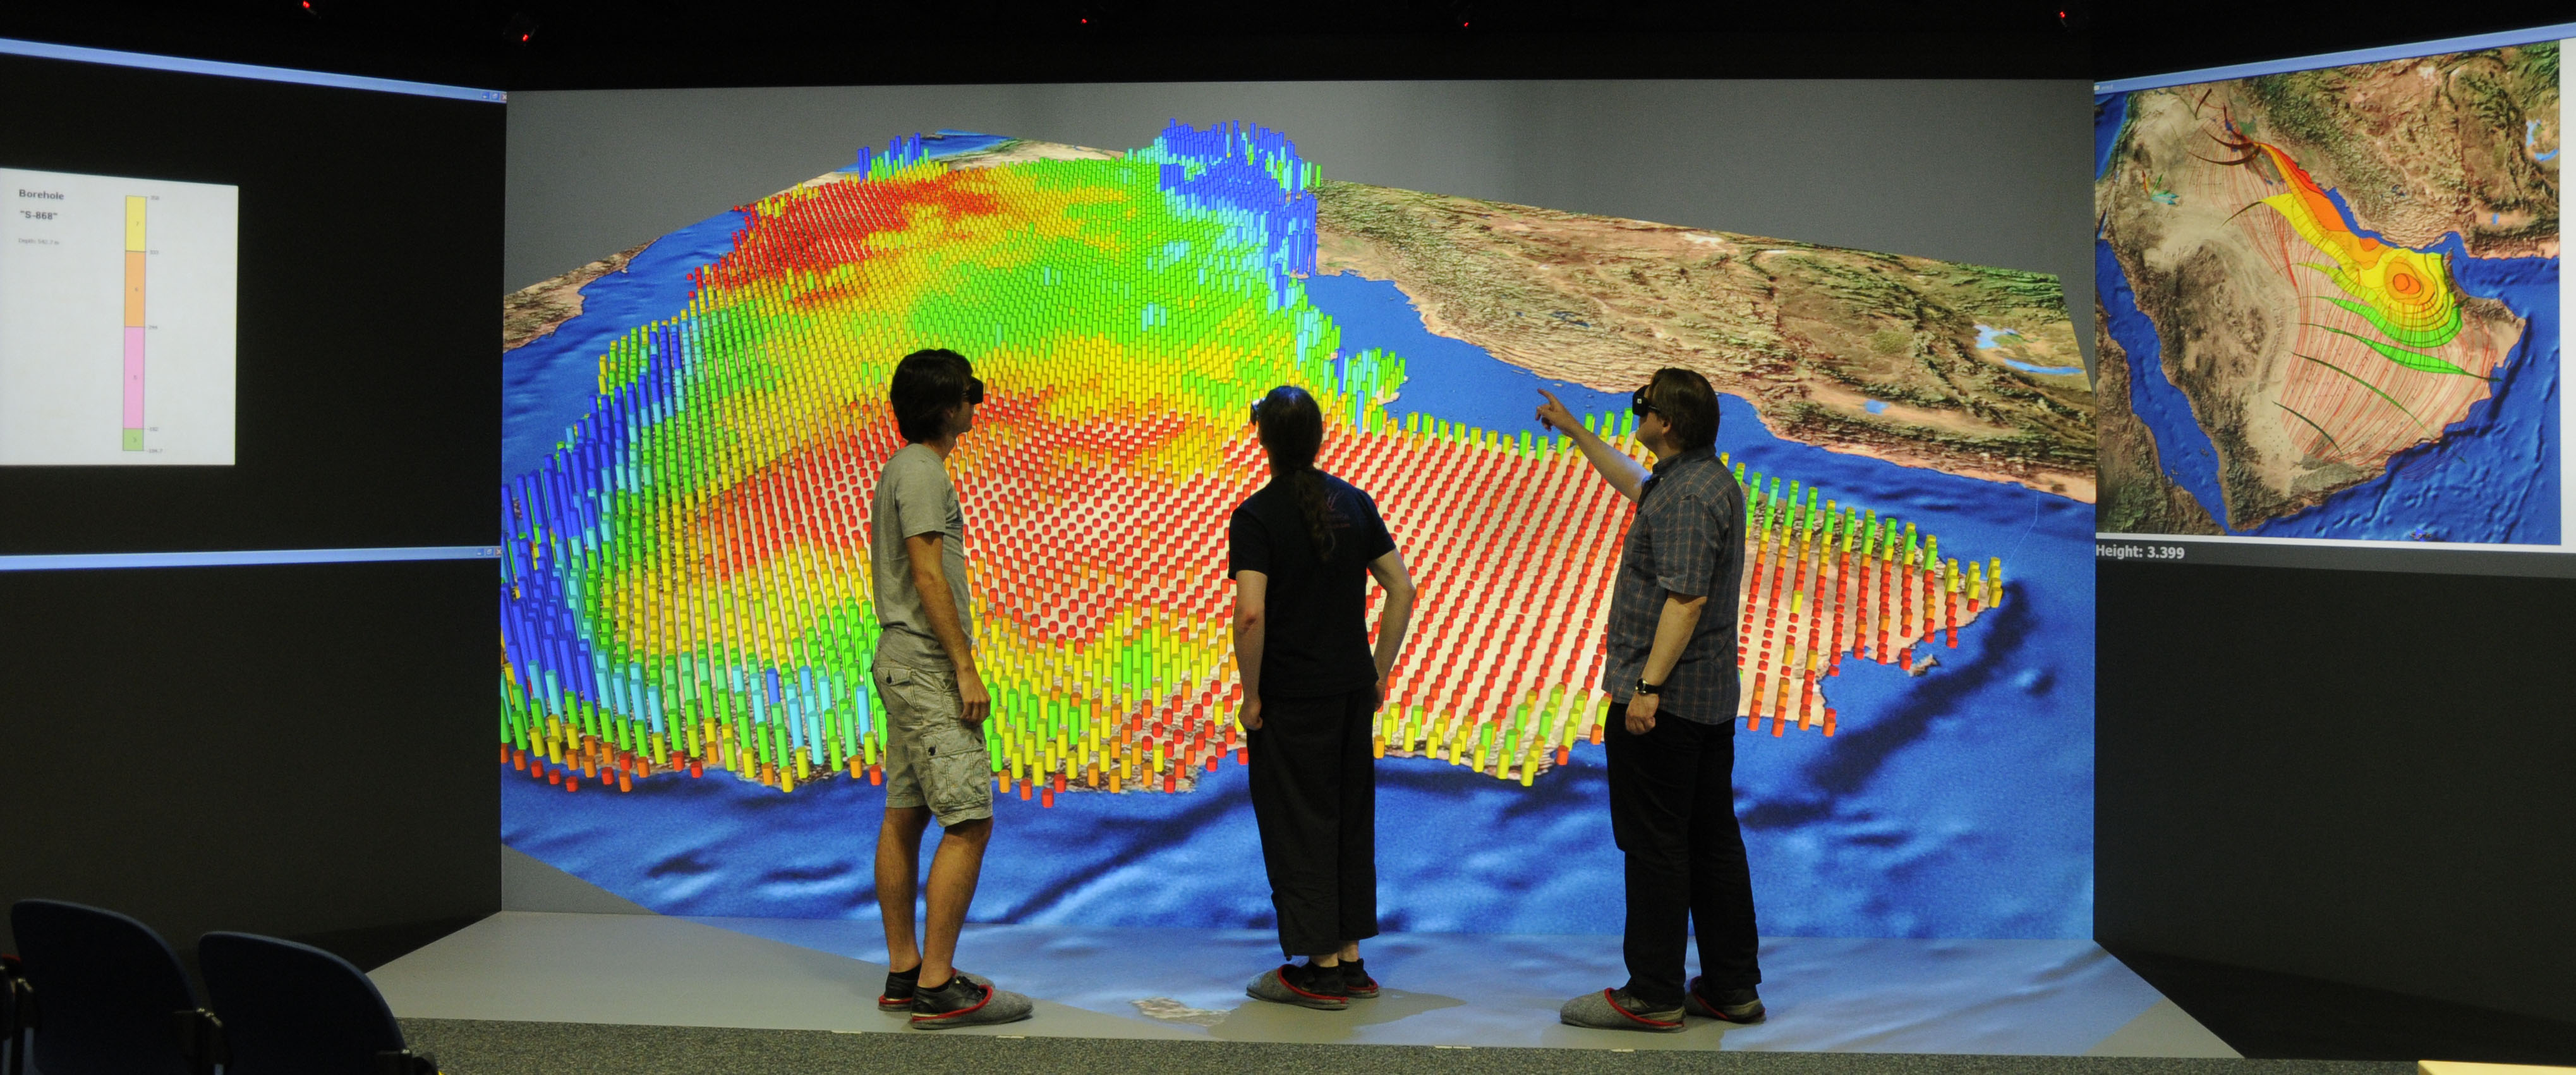
\includegraphics[width=1.0\textwidth]{images/sa_2d_3d.jpg}
\caption{Mixed 2D / 3D visualization of observed rain events on the Arabian Peninsula~\cite{rink:iwas}. In addition to the stereoscopic image on the main screen, stratigraphies from interactively selectable borehole data (on the left) and an overview map (on the right), indicating the current observer position, are shown.}
\label{fig:sa}
\end{figure*}

\subsection{Mobile VR equipment}
\label{mobile-vr-equipment}

For off-site presentations such as on conferences, workshops or visits to project partners or stakeholders, we can also utilize mobile equipment to demonstrate the same visualization projects as in the \emph{VISLab} (although in a much smaller resolution and also limited to one concurrent user). The equipment consists of notebooks with dedicated GPUs and stereoscopic projectors or head-mounted displays such as the \emph{Oculus Rift}~\cite{web:rift} as shown in figure \ref{fig:rift}.

\begin{figure}[htb]
  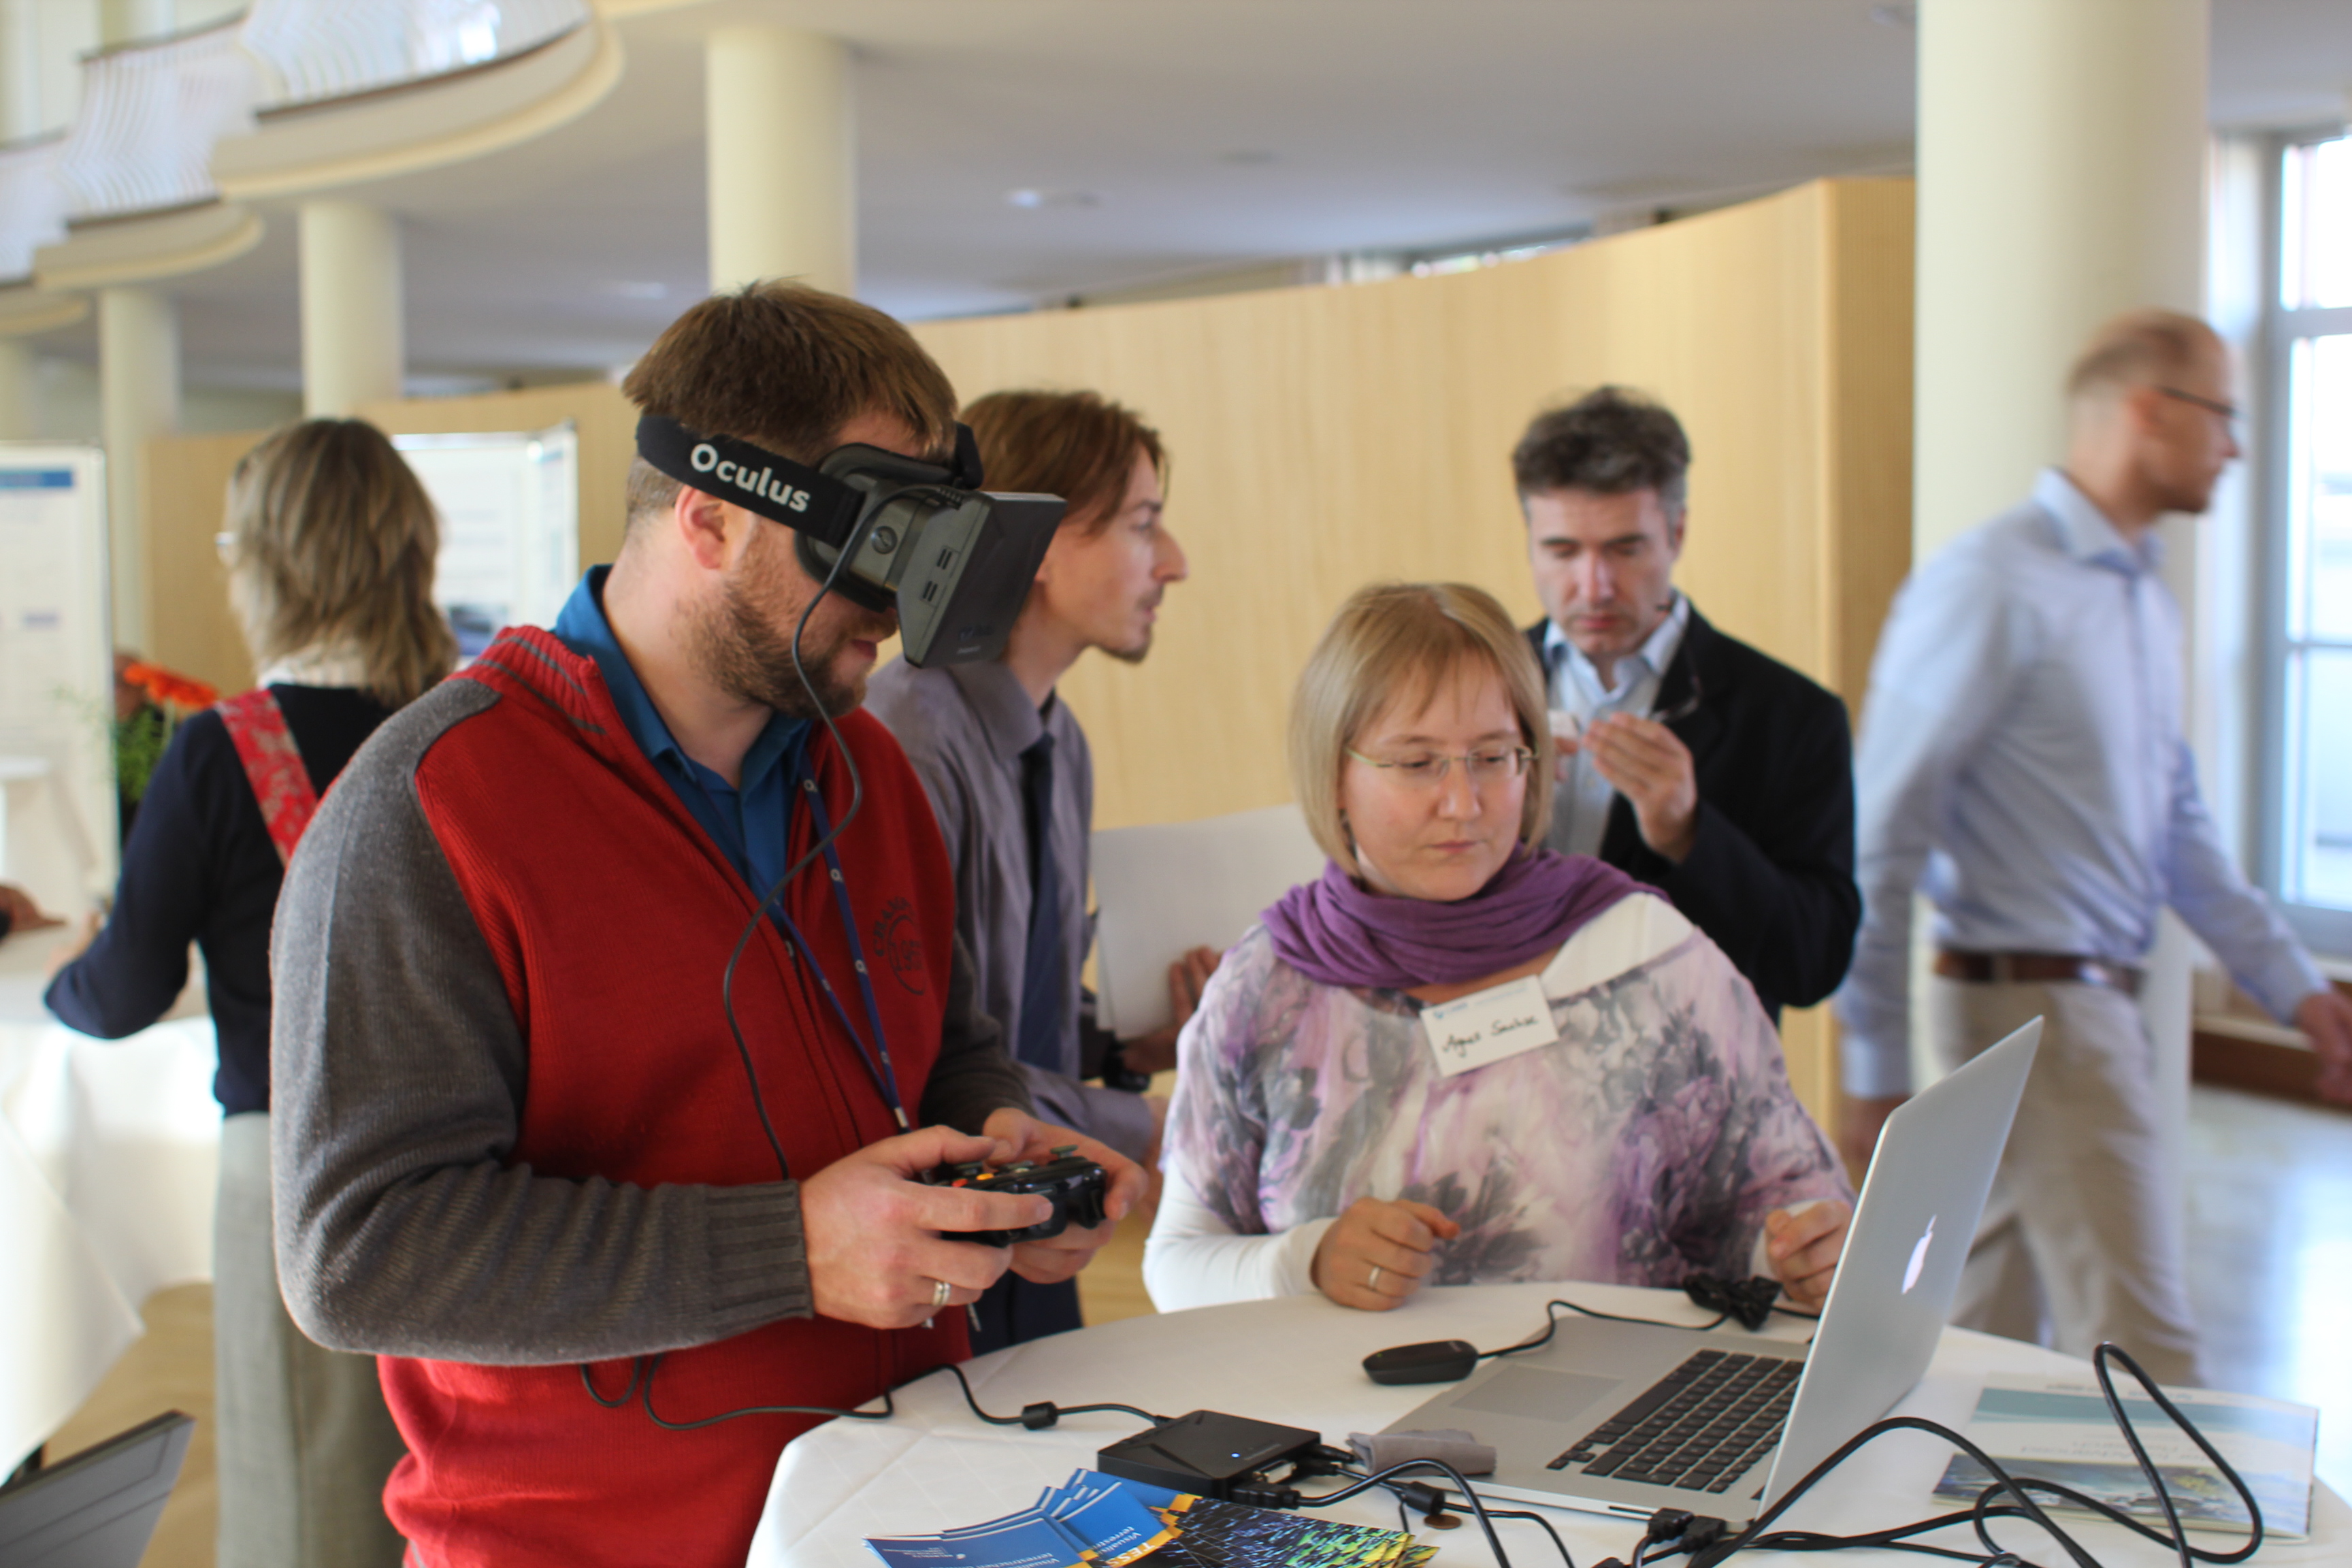
\includegraphics[width=\linewidth]{images/rift.jpg}
\caption{Mobile presentation with help of a head-mounted display and a game console like input controller at a scientific conference.}
\label{fig:rift}
\end{figure}

\subsection{Software}
\label{software}

Because of the clustered setup, we can only use software which can run in parallel and synchronizes the current state across all involved machines. There are specialized software with integrated cluster rendering capabilities and middleware software which add this functionality on top of non-clustered applications. These middlewares, such as \emph{Techviz}~\cite{web:techviz} or \emph{Conduit}~\cite{web:conduit}, intercept graphic commands from a desktop application and redistribute them to a render cluster. Such middleware software products allow to run a regular 3D desktop application in a VR environment with stereoscopy and tracking enabled. A data conversion is not necessary for this setup but interaction and presentation techniques are limited by the desktop application employed and performance is lost during graphic commands interception and distribution to the cluster such that immersion and feedback are severely affected.

Due to these disadvantages, we use software packages with native cluster rendering capabilities such as \emph{VRED}, \emph{ParaView} or \emph{Unity} in conjunction with \emph{MiddleVR}. All of these are introduced in the following:

\paragraph{VRED}
is a commercial software by \emph{Autodesk} (former \emph{PI-VR}) specialized in photorealistic real-time product rendering running on Windows~\cite{web:vred}. It is build on top of \emph{OpenSG}, an open-source scene graph library which offers clustered rendering~\cite{opensg}. \emph{VRED} can arrange imported 3D objects in a virtual scene, allows for tweaking of material (properties how the surface of the 3D objects reacts to lighting) and lighting parameters but is neither a modeling software nor are there many interaction possibilities besides viewer movement and object selection. It has a plug-in interface but no documentation is available from the vendor on how to address it. An advantage of the software is that \emph{VRED}'s editor can be directly connected to the \emph{VISLab}'s display so that local changes to the scene done at the presentation terminal are visible immediately on the video wall.

\paragraph{ParaView}
is an open-source data analysis and visualization software~\cite{paraview} by \emph{Kitware Inc.} build on top of the \emph{Visualization Toolkit}~\cite{vtk} (\emph{VTK}). Both technologies are also integrated in our visualization workflows (see \ref{workflows}). \emph{ParaView} allows to quickly create visualizations and implements a large number of well established visualization algorithms and techniques. It can run on distributed memory architectures to analyze large data sets and to drive VR displays. Using \emph{ParaView}, we can modify visualization parameters directly in the VR environment. Unfortunately, it lacks more sophisticated interaction and presentation features.

\paragraph{Unity}
is a complete game engine by \emph{Unity Technologies}~\cite{goldstone:unity3d}. It is available in a free and a commercial editor variant with the latter supporting more advanced rendering techniques (soft shadows, HDR, post-processing effects) and team collaboration features. \emph{Unity} has several rendering backends (\emph{OpenGL}, \emph{OpenGL ES}, \emph{Web\-GL}, \emph{DirectX}) so it can be run on all major platforms as well as on the Web (with an additional browser plug-in)~\cite{web:unity}. \emph{Unity}'s basic scope of operation does not include any interaction functionality but it has a comprehensive scripting documentation and a vivid plugin community so that it is very easy to integrate missing features. Application testing can be done directly in the \emph{Unity} editor by tweaking the application at runtime. However, \emph{Unity} created applications cannot run in a clustered environment. Therefore \emph{MiddleVR} is used.

\paragraph{MiddleVR}
is a generic virtual reality middleware from \emph{i'm in VR} designed to work with different 3D applications~\cite{web:middlevr}. It features a graphical configuration tool to setup VR systems independent of specific software. It implements interaction devices, stereoscopic rendering and clustering when using software not supporting this functionality. The \emph{MiddleVR} configuration is then used in a \emph{Unity} plugin to enable all these features in Unity applications. The \emph{MiddleVR}-enabled Unity application is VR system agnostic, once compiled it can be run on any VR system supported by \emph{MiddleVR}. A disadvantage of this approach is that the final application cannot be run inside the Unity editor but stand-alone, so that it cannot be altered interactively at runtime. The fact that a recompilation of the application takes just a few seconds weakens that drawback.

For the future, we will focus on the use of Unity as a platform for highly interactive visualizations to illustrate and discuss complex phenomena. In contrast, ParaView is more suited for rapid prototyping and exploration of complex data sets but will also play an important role in future workflows (see \ref{in-situ-visualization}).

\subsection{Workflows}
\label{workflows}

For simulation, we employ \emph{OpenGeoSys}~\cite{kolditz:ogs}, an open-source platform and flexible numerical framework for the simulation of thermo-hydro-mechanical / chemical processes in porous and fractured media with applications in geoscience and hydrology. In order to simulate these processes models are defined that include as much relevant data as possible to account for all phenomena defining that natural system. Heterogeneous data sets representing the model characteristics are given as input parameters to the simulation software which returns result data sets predicting system behavior in areas of interests.

We are both using visualization when setting up the model and simulation as well as to analyze simulation result data. As a basis for creating visualizations we employ \emph{VTK} which is also integrated into the \emph{OGS Data Explorer} framework (a data integration and visualization tool for pre- and postprocessing \emph{OpenGeoSys} simulation data~\cite{rink:eesenvirvis}) as well as \emph{ParaView}.

We provide utilities and \emph{ParaView} plugins to convert \emph{VTK} visualization data to formats supported by the VR frameworks used in the \emph{VISLab}, i.e.~OpenSG for \emph{VRED}~\cite{bilke:vtkosgconverter} and Autodesk FBX for \emph{Unity}~\cite{bilke:vtkfbxconverter}. Conversion can be either done manually in the \emph{OGS Data Explorer} or in a batch process by employing \emph{ParaView}'s Python scripting interface. The second approach is especially useful when converting large sequences of complex data sets such as time steps of simulation results from transient finite element models. During conversion, meta data is appended to the data sets to include information not necessarily supported in FBX such as a specific material and rendering setup or time stepping information. This meta data is evaluated when loading the data sets into Unity and can be queried, i.e.~for displaying the time stepping information as a text overlay. Multiple data sets can be arranged both in a spatial but also in a temporal context and a variety of presentation techniques (i.e. defining camera animations, fading in/out of data sets, selection of subsets, displaying additional information) are implemented, see~\cite{rink:eesenvirvis} for details.

\section{Overview of VISLab applications}
\label{overview-of-VISLab-applications}

In the following, several case studies are presented which used our visualization workflows and utilized the \emph{VISLab}. Most of them have a background in hydrology, geosciences or energy but research projects furthermore include topics in urban planning and climate prediction.

\subsection{Ammer catchment}
\label{ammer-catchment}

The catchment of the river Ammer in southwest Germany has been selected as the study region for a holistic analysis of the water cycle coupled to reactive solute transport, for addressing water and solute fluxes at the catchment scale as a function of and in feedback with changes in climate, land use, and water usage~\cite{grathwohl:wessti}. The river has a length of 25\,km and is a tributary to the Neckar. Its catchment has a size of 180\,km\textsuperscript{2} with a geology comprised of a sequence of Triassic strata forming a landscape characterized by escarpments~\cite{selle:wessti}. The Ammer is mainly fed by groundwater from the karstic and fractured aquifers and drains the catchment at a rate of ca. $1\,m^3/s$.

The finite-element groundwater model is based on a digital elevation model with a resolution of 100\,m in combination with interpolated subsurface layers based on the stratigraphic data of over 100 boreholes. For simulation purposes, the subsurface information has been combined into four separate layers, consisting of a part\-ly karstified limestone aquifer overlaid by Keuper-layers. In addition, the scene includes the stream network and groundwater production wells, which are employed as boundary conditions for the model as well as raster data with groundwater recharge information. Based on the results of a steady-state groundwater recharge simulation, the presentation also includes iso-surfaces representing the groundwater head as well as stream tracers for the visualization of flow paths within the catchment. See ~\cite{selle:wessti} for more information on the groundwater study and~\cite{rink:wessti} for model setup and data visualization.

\subsection{Western Dead Sea -- Sustainable management of water in arid and semi-arid regions}
\label{western-dead-sea---sustainable-management-of-water-in-arid-and-semi-arid-regions}

\begin{figure}[htb]
  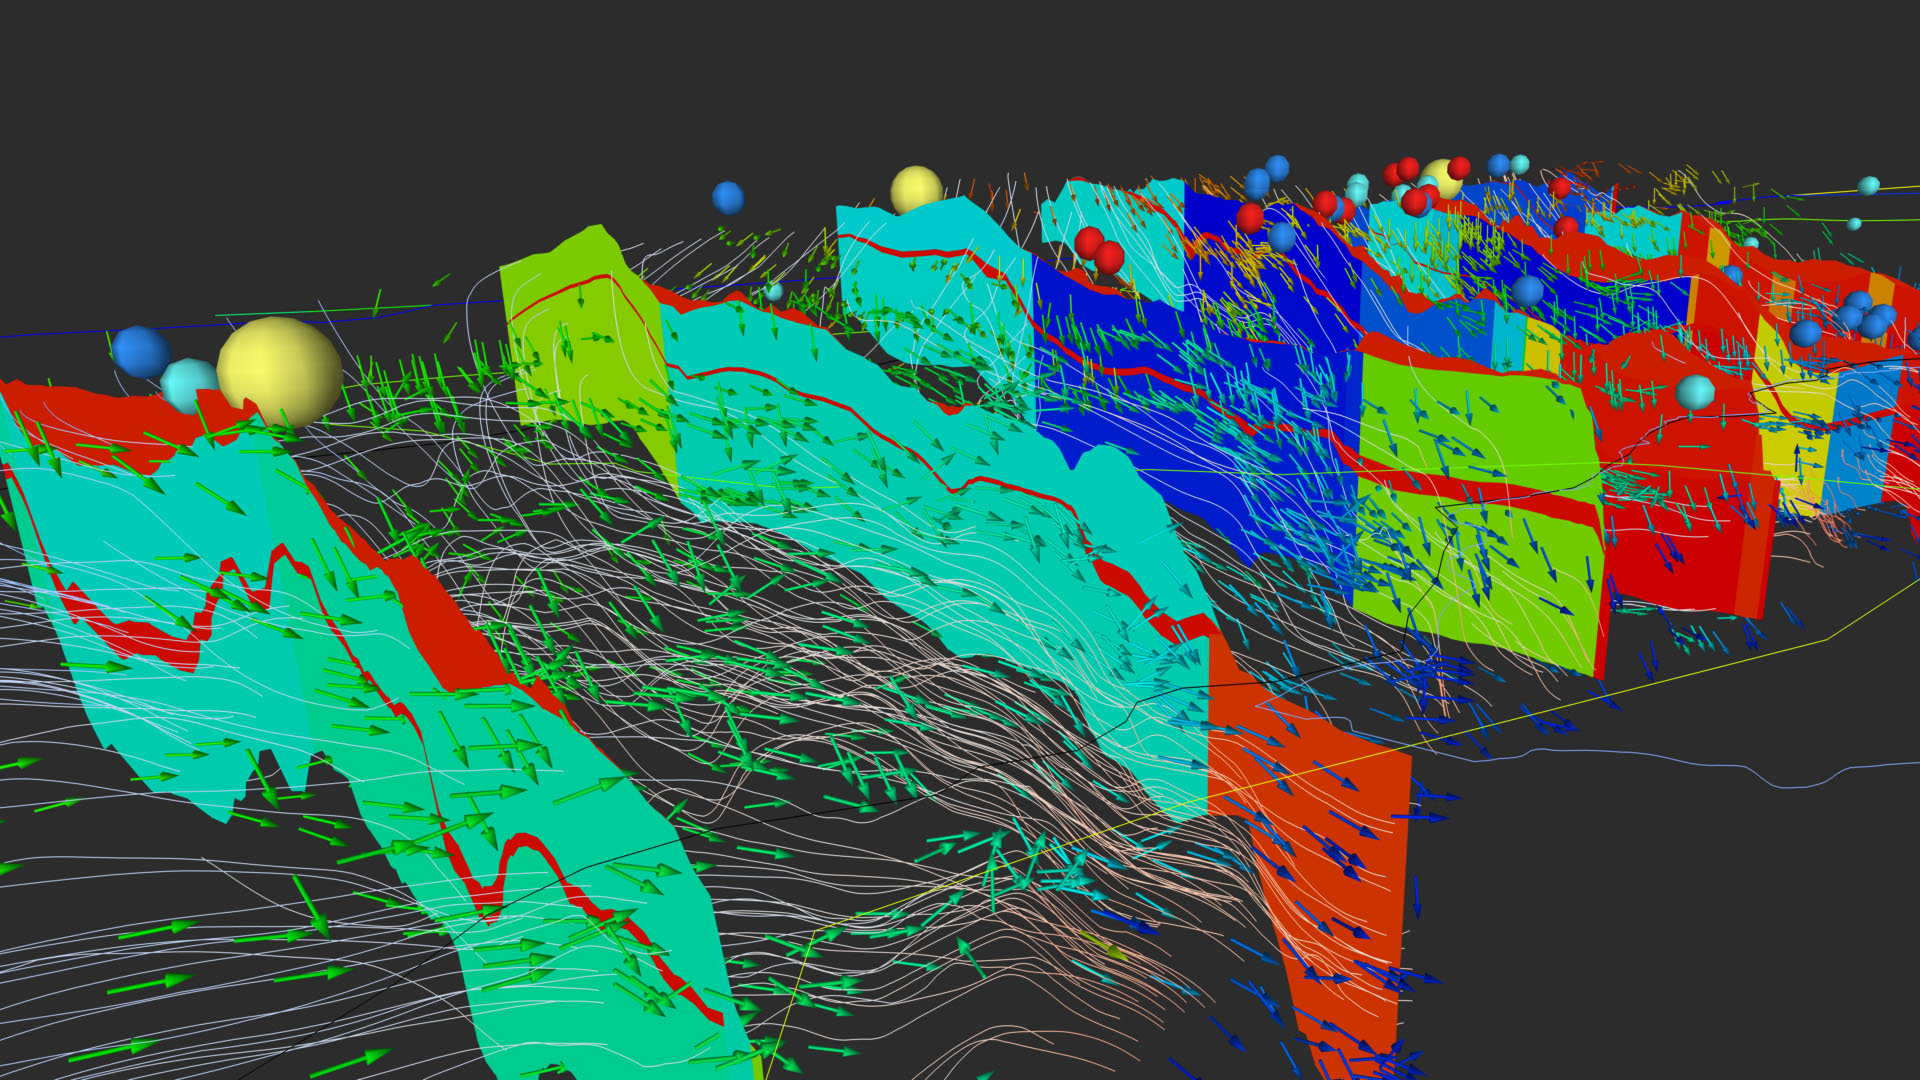
\includegraphics[width=\linewidth]{images/deadsea.jpg}
\caption{Cross section of the Upper and Lower Judea Group aquifer of the Western Dead Sea catchment, divided by an thin aquiclude (red line). The density of the groundwater flow paths with its velocity vectors describes the groundwater flow dynamics of the Cretaceous aquifer system from west of the catchment towards the Dead Sea. Colored spheres show the locations of wells, climate stations and cities for better orientation.}
\label{fig:deadsea}
\end{figure}

The catchment of the Western Dead Sea (Israel / Palestine) was analyzed within the \emph{SUMAR}-Project and de\-mon\-strates a groundwater flow model of a semi-arid to arid case study which is coupled with a hydrological model. The climatic conditions exacerbate the tense situation of the drinking water supply for the 3800\,km\textsuperscript{2} large study area. And secondly, they lead to political and socio-environmental stresses. The overall aim of the \emph{SU\-MAR}-project~\cite{Siebert:2014} focuses on the quantity of surface and groundwater fluxes inside the catchment, which is influenced by faults of the Jordan Rift Valley System and were drained towards the shrinking, hypersaline and endoheric Dead Sea.

Several methods were applied to localize (with remote sensing data), to quantify (with 2D hydrological and 3D groundwater flow modeling) and to simulate water flow volumes and flow paths (with groundwater flow modeling~\cite{graebe:modelcare}) towards the Dead Sea. The study area is characterized by two Cretaceous limestone aquifers (confined / unconfined) of around 400\,m thickness including steep hydraulic gradients, which serve as the only fresh water resources in this region. Especially the visualization of the numerical groundwater flow model (see figure \ref{fig:deadsea}), which was implemented into OpenGeoSys, helps to detect uncertainties of the hydrogeological input data sets and enables a comprehension of the flow dynamics of the heterogeneous partly karstified limestone aquifer. To this end the calibrated steady state groundwater flow model provides quantifications of the water balance of the subsurface catchment and is the starting point for the transient modeling of surface and subsurface flow processes~\cite{graebe:wessti}. The hydrological model \emph{J2000g}~\cite{KrauseKralisch:2005, Krause:2001} was applied to estimate i.e.~the groundwater recharge of the widely distributed bare rock soil cover for a 30 years period. Its result was transferred as a time dependent boundary condition to the 3D finite element mesh nodes with a resolution of 250\,m and represents by its trend the continuous lowering of the water level in the aquifer system due to over pumping issues.

\subsection{Nankou -- Groundwater deterioration in a suburban area of Beijing}
\label{nankou}

\begin{figure}[htb]
  \includegraphics[width=\linewidth]{images/nankou.jpg}
\caption{A simulated ground water flow system is shown around pumping wells in the Nankou area with nitrate concentrations as colors on the streamlines.}
\label{fig:nankou}
\end{figure}

Nitrate contamination of groundwater resources is a severe environmental problem worldwide, mostly caused by extensive agriculture using large amounts of fertilizer to increase plant productivity. Nitrate has extreme long residence times in the subsurface and remediation is therefore hampered and requires costly long-term efforts. Therefore, simulation and visualization are important tools for planning and optimization of remediation scenarios. Figure \ref{fig:nankou} depicts the visualization of an OpenGeoSys subsurface model for the development of remediation setups of nitrate contaminations in China (\emph{Nankou} project) using the VR environment of the \emph{VISLab}. To present complex hydro-geological structures and results of nitrate remediation in the Nankou area to stakeholders and decision-makers of the Beijing district, 3D visualization techniques have been successfully used to foster both understanding and discussion of the invoked environmental problems within the geographical context, data availability and simulation results for the Nankou nitrate remediation project in China~\cite{sun:ees}.


\subsection{Oman -- Saltwater intrusion modeling}
\label{oman---saltwater-intrusion}

Within the project \emph{International Water Research Alliance Saxony} (IWAS), one of the main goals was to assess and evaluate water resources under various natural and human induced stress conditions. Several subprojects considered study regions in different parts of the world~\cite{kalbus:ees}.

\begin{figure}[htb]
  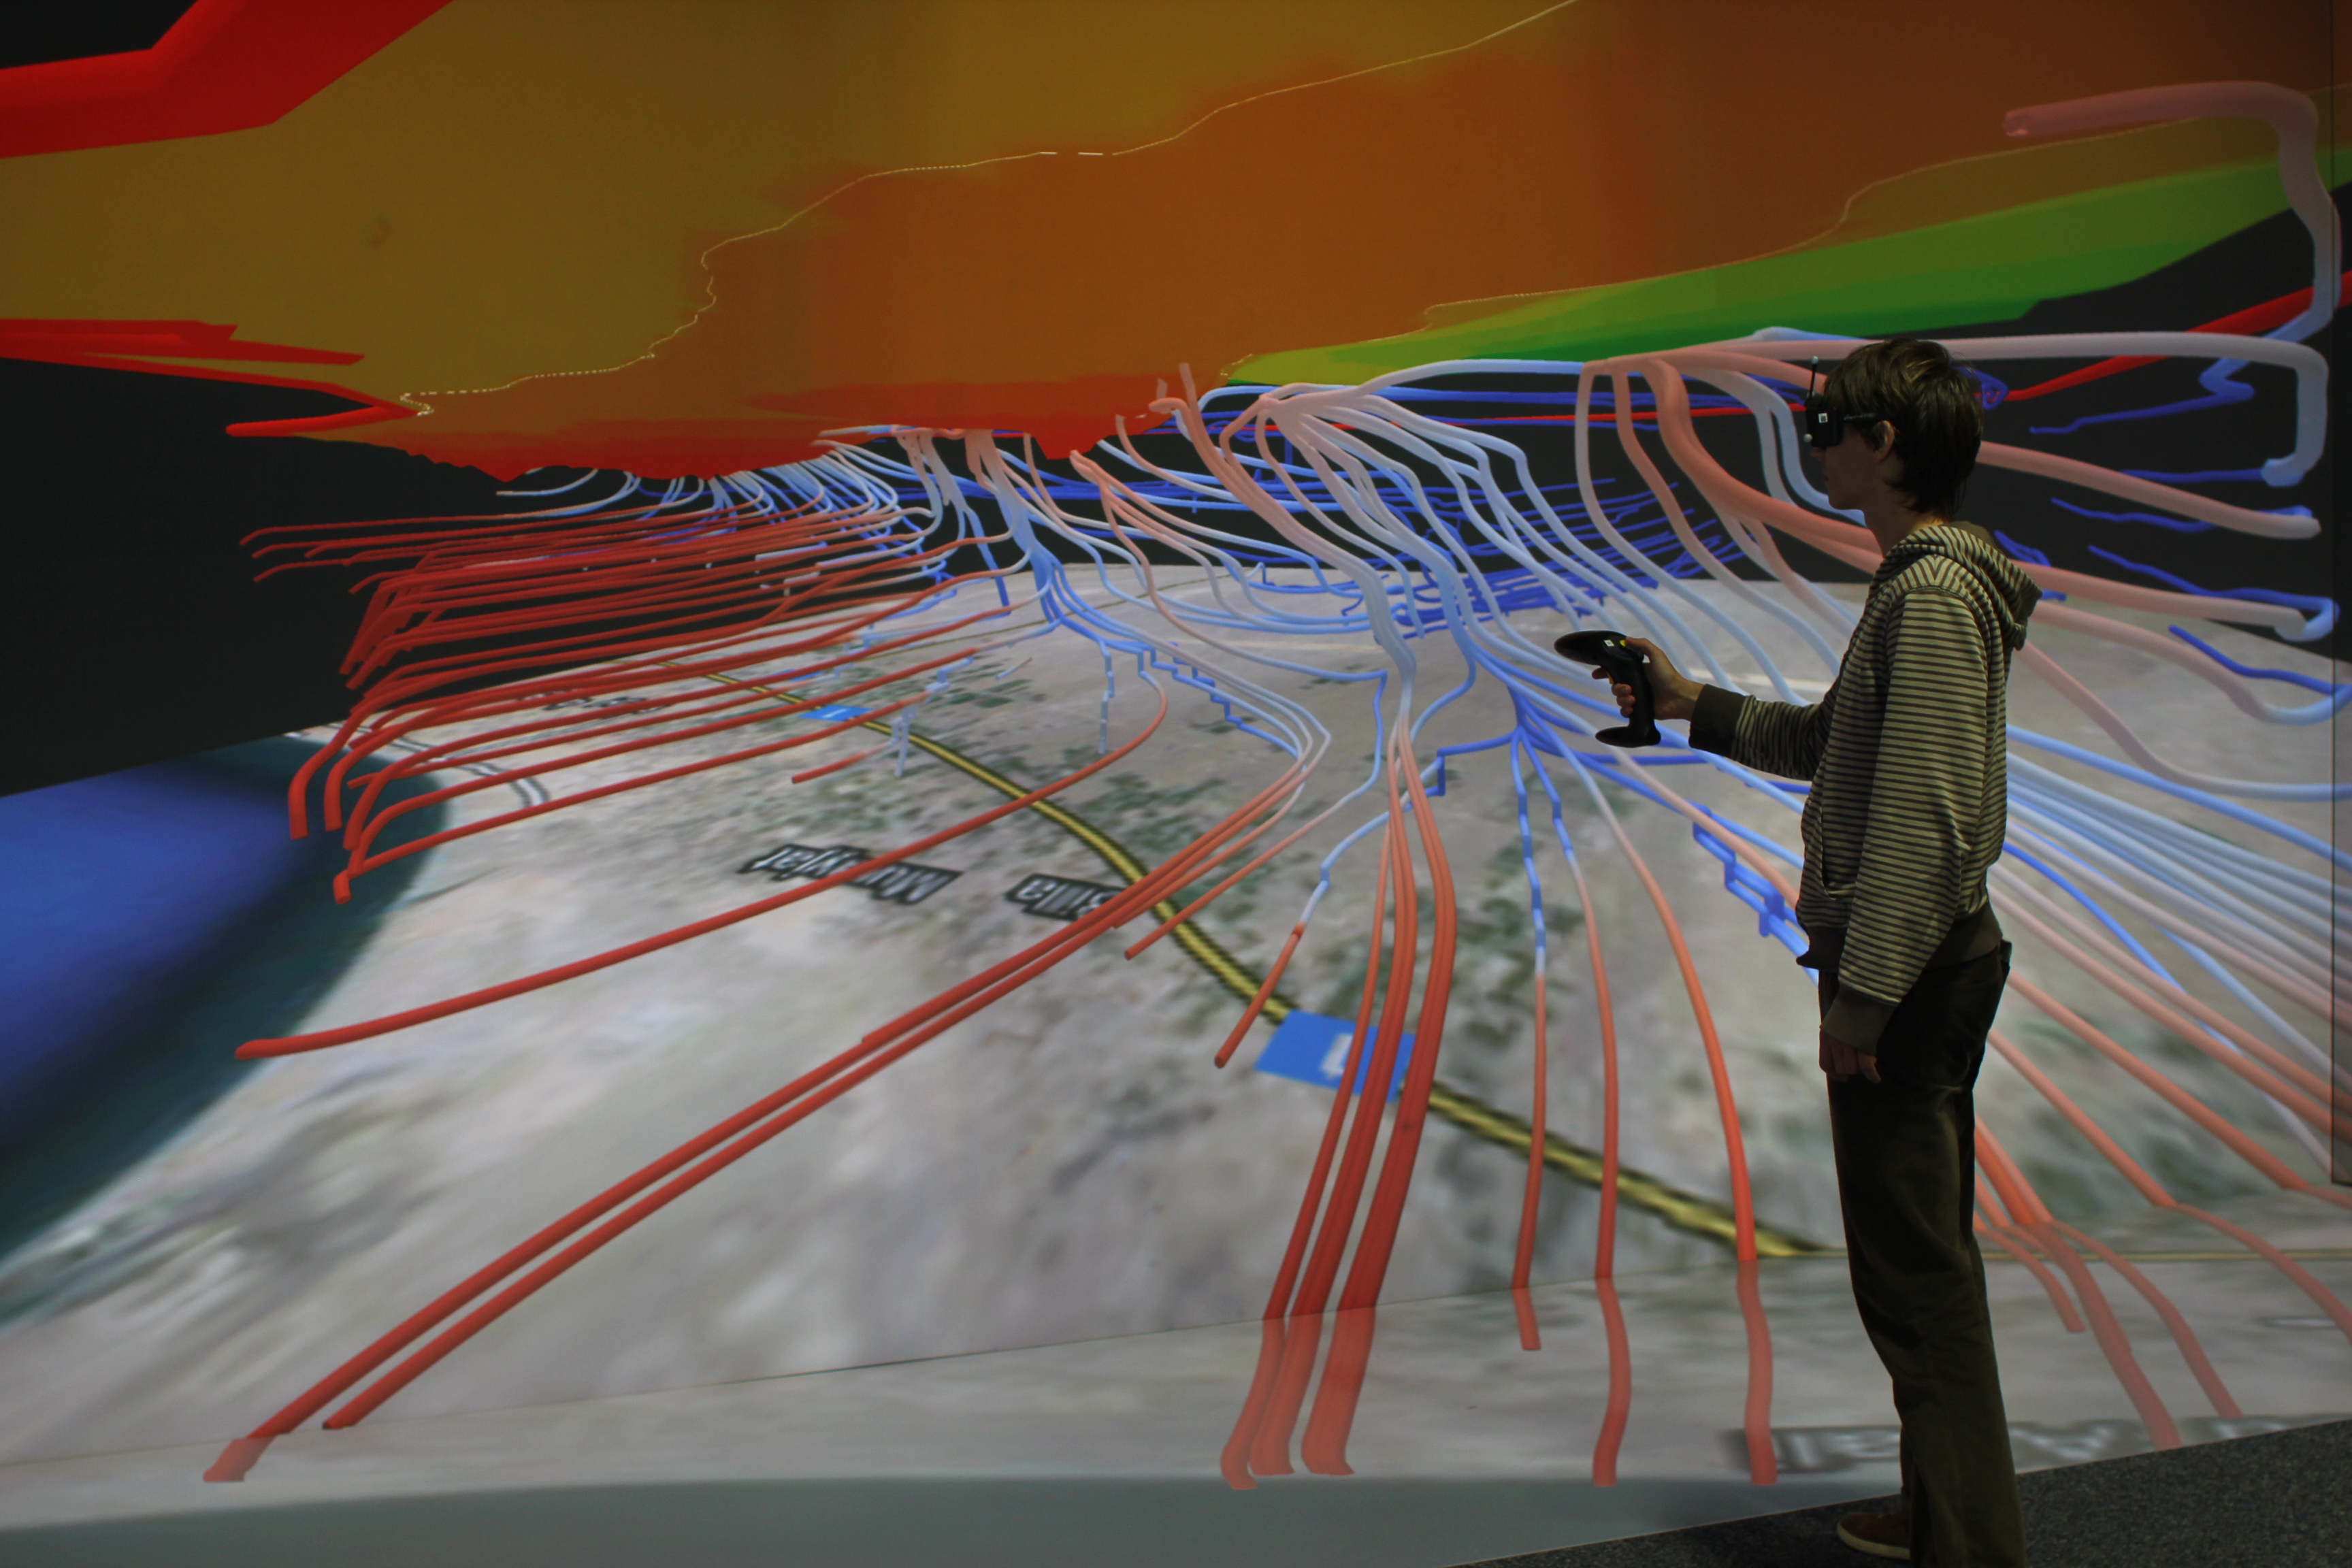
\includegraphics[width=\linewidth]{images/oman.jpg}
\caption{Analyzing groundwater flow patterns at the near coastal salt/freshwater interface (red/blue color on streamlines) in combination with groundwater surface drawdown due to pumping activities for determining subsurface water vulnerabilities utilizing the stereoscopic mode of the VISLab.}
\label{fig:oman}
\end{figure}

One of these case studies, a region scale study on density driven flow in a coastal aquifer that is used as source for agriculture irrigation, intensively made use of visualization options during model setup, verification of the variable density process~\cite{Beinhorn200589}, and for the transfer of knowledge to local authorities~\cite{walther:cam, walther:eesenvirvis}. Firstly, visualization was used to investigate plausibility of the set up hydro-geological model, that was constructed based on an extended inverse weighting distance interpolation~\cite{walther:modelcare}. Secondly, large data sets of model calibration and long term scenario simulations of the saltwater intrusion process were analyzed by utilizing \emph{ParaView}. \emph{ParaView} was run on a parallel cluster computer to omit bandwidth limitations to copy large data and to reduce computational burden on standard desktop machines. Thirdly, results of the modeling were visualized, which helped during discussions with experts and tremendously aided in knowledge transfer during a visit of Omani authorities from the Ministry of Regional Municipalities and Water Resources. Additionally, throughout all states of model development, calibration, scenario analysis, and result presentation, the \emph{VISLab} was utilized~\cite{walther:eesenvirvis}.

\subsection{TERENO -- Observatory Harz/Central German Lowlands}\label{tereno-bode}

\begin{figure}[htb]
  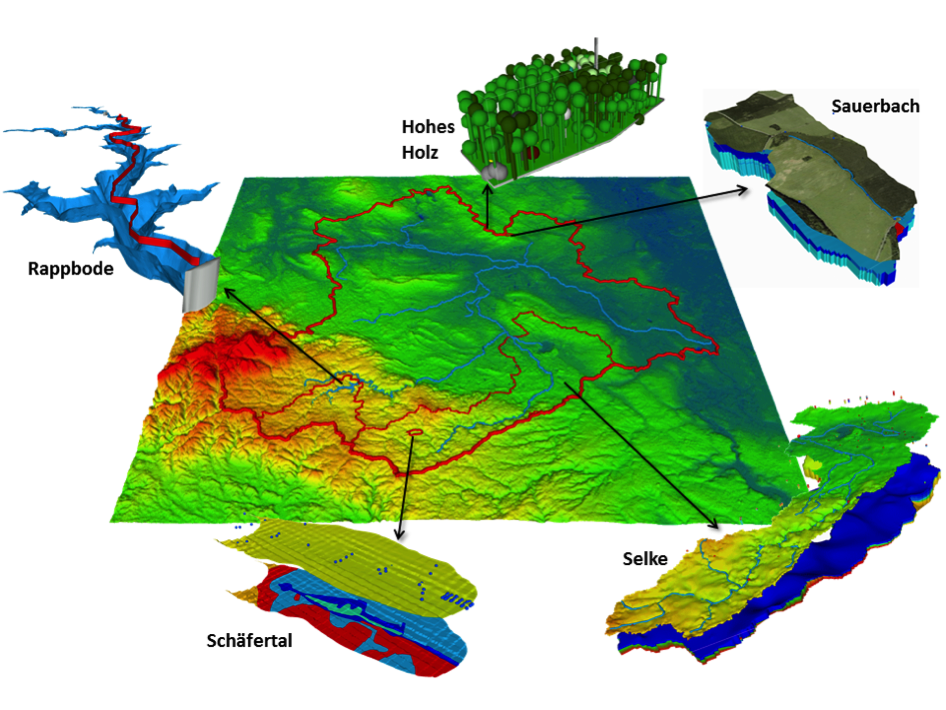
\includegraphics[width=\linewidth]{images/tereno.png}
\caption{Visualization of the Bode catchment (bold red lines) of the TERENO investigation based on a digital elevation model (DEM) including the intensive test sites, Rappbode reservoir \cite{rinke:ees}, Hohes Holz, Sauerbach, Selke catchment hosting the Sch\"afertal.}
\label{fig:tereno}
\end{figure}

TERENO is a large-scale project aims to catalogue the longterm ecological, social and economic impact of global change at regional level~\cite{zacharias:tereno}. Four areas in Germany have been selected and are now heavily instrumented to allow extensive studies and simulations for researchers from different disciplines. Hydrogeological analysis in central Germany is being conducted in the catchment of the River Bode with a size of 3,100\,km\textsuperscript{2} (see figure \ref{fig:tereno}). Within that area a number of intensive test sites have been selected, ranging in size from a small area of about one hectare, concerned with assessment of water balance in a forested region, to the complete catchment of one of the Bode's tributaries with a size of over 450\,km\textsuperscript{2} where hydrological processes in the stream as well as in the hyporheic zone are investigated~\cite{schmidt:selke, trauth:flow} as shown in figure \ref{fig:streambed}.

\begin{figure}[htb]
  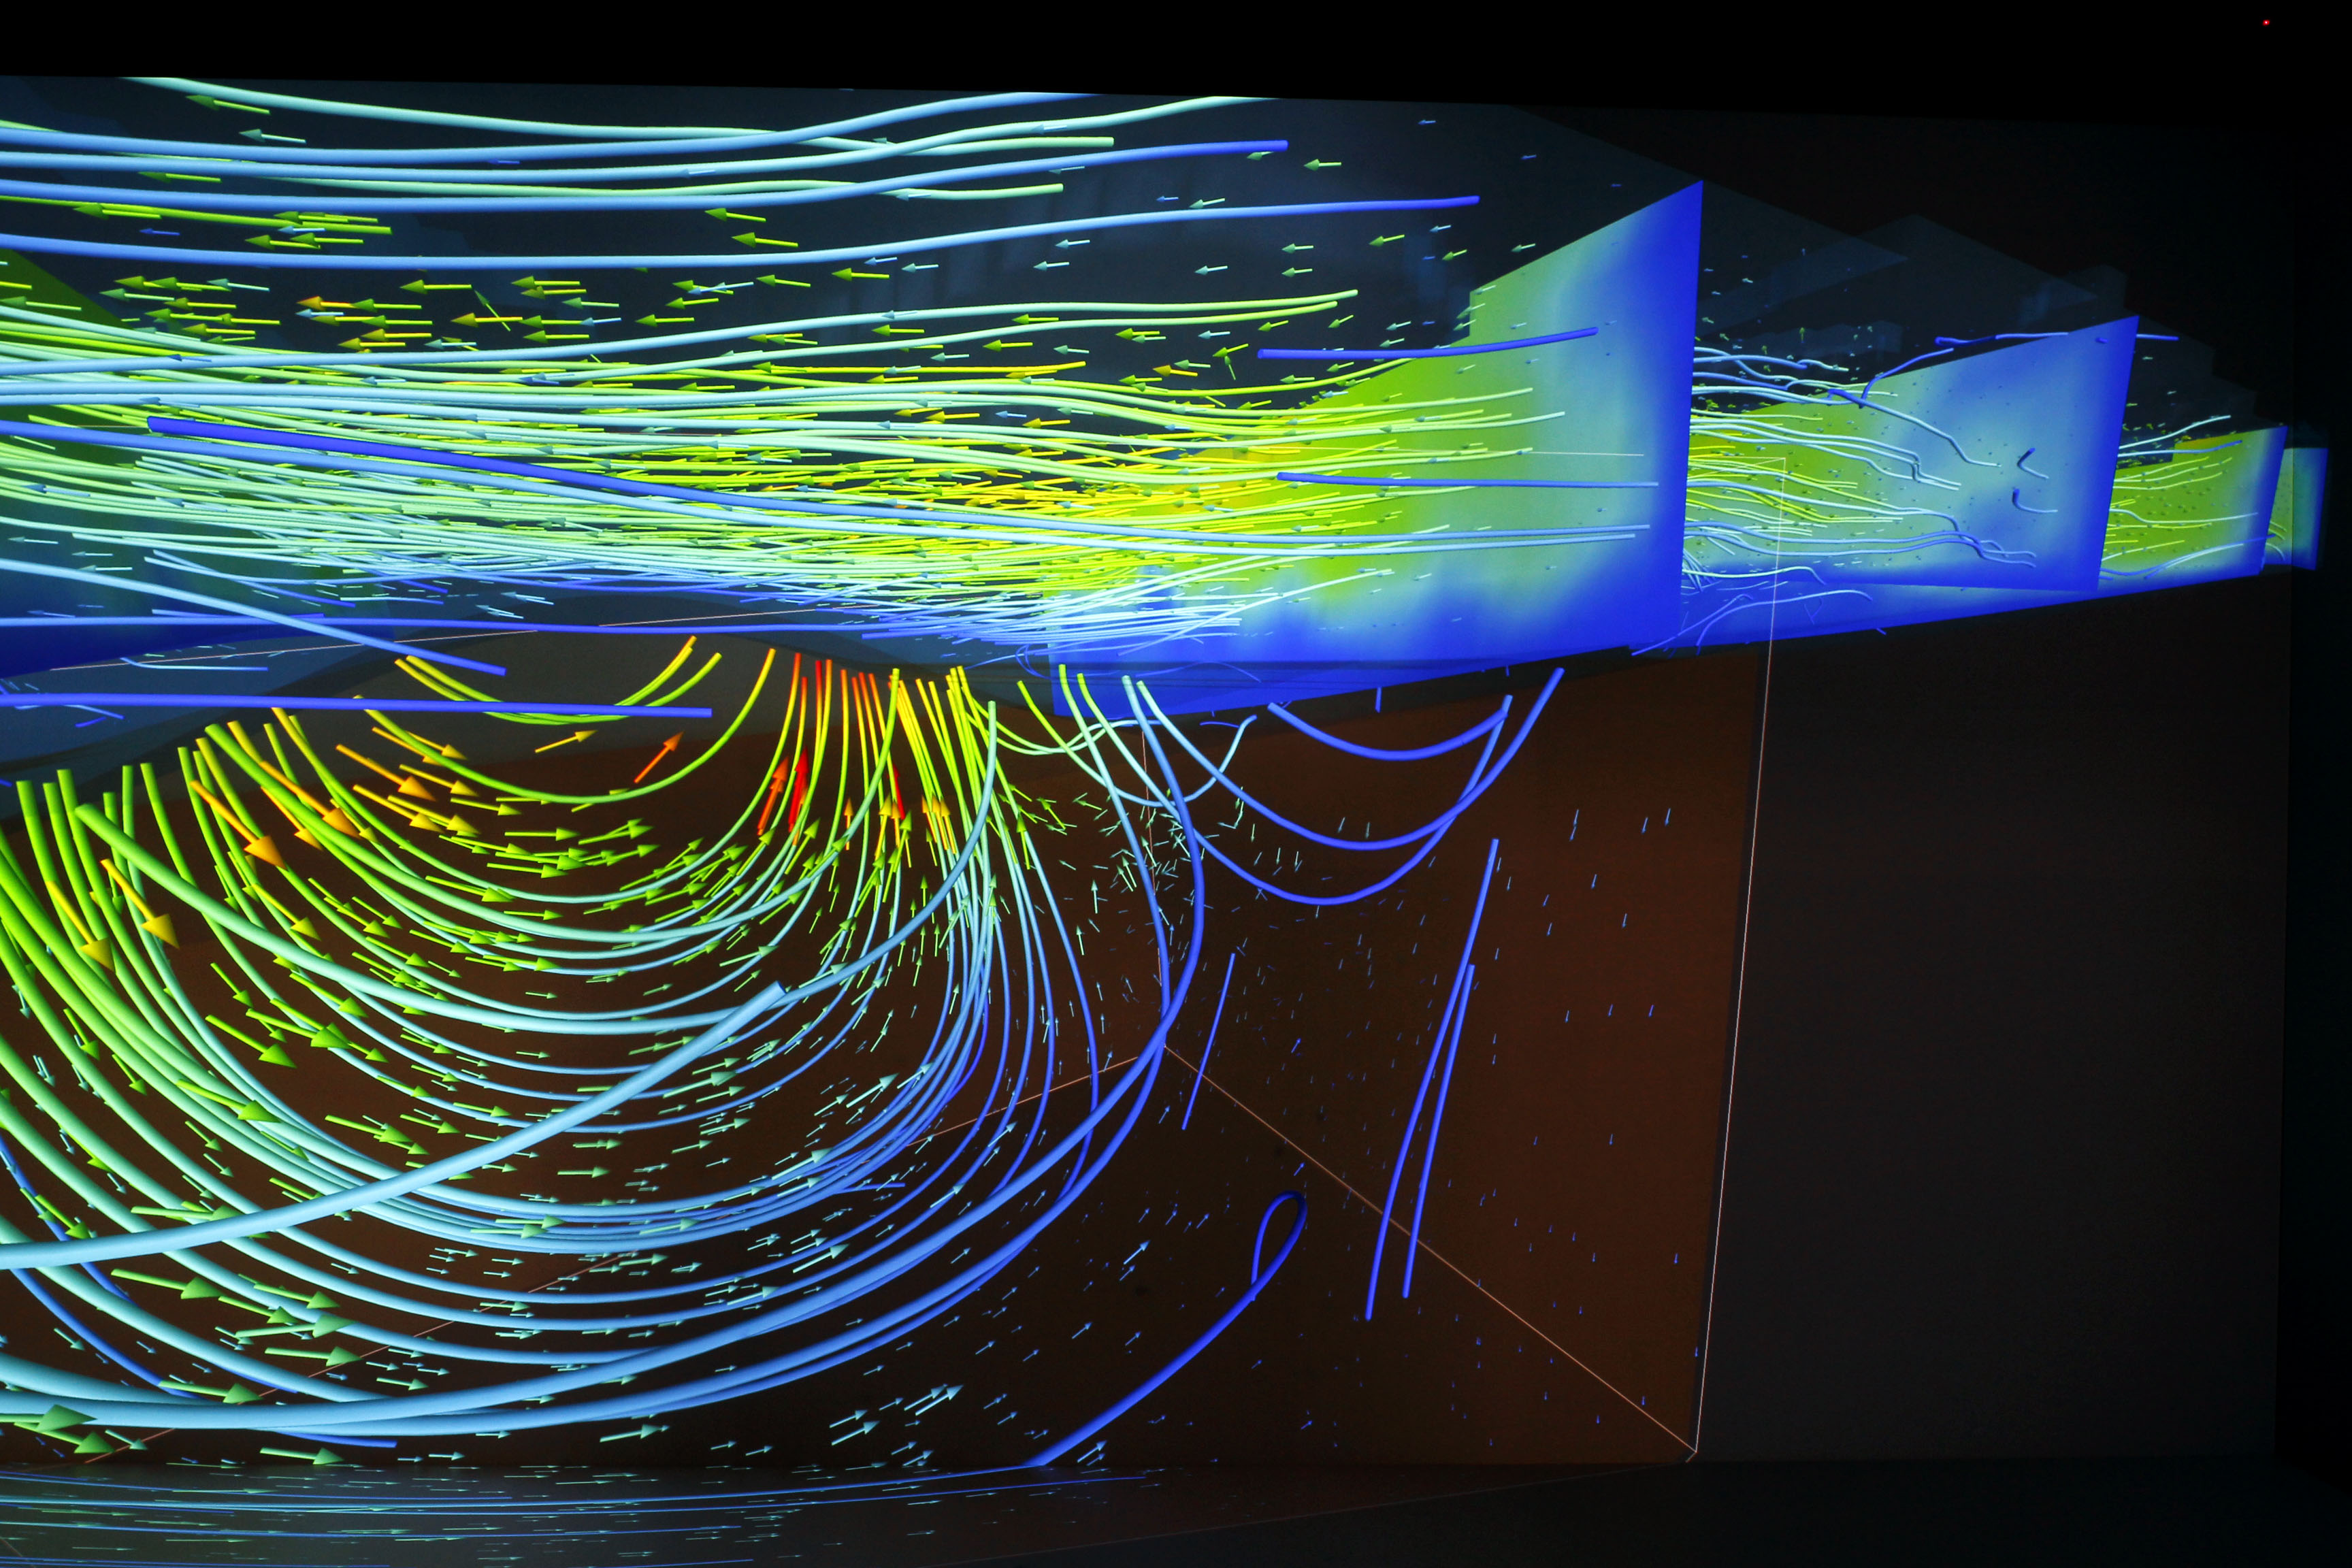
\includegraphics[width=\linewidth]{images/streambed.jpg}
\caption{Liquid flow turbulences in a streambed (top) are concurrently visualized with water intrusion in the underground forming a ground water flow system (bottom).}
\label{fig:streambed}
\end{figure}

The presentation consists of over $70$ heterogeneous data sets of different scale and resolution. Most notable are surface representations, consisting of a terrain model of the whole region with over 1 mio triangles with a max edge length of 30\,m. Terrain models of the intensive test sites also exist at a much finer resolution, ranging from 30\,m for the larger regions to just 1\,m for the regions covering 1\,km\textsuperscript{2} or less. Various color transfer functions or textures can be applied to these surfaces, including elevation information, soil moisture, or indication of land use. While textures are originating from raster data, transfer functions are based on statistical data or look-up tables. Geometrical information includes the courses of streams at various resolutions and displayed with different prominence. Furthermore, the scene includes climate stations, measurement networks, bathymetries of some of the larger water bodies within the region, structural models for the subsurface of two intensive test sites, borehole data and much more. Most regional data sets are only visible when the presentation zooms in on the intensive test site they are located in, to avoid unnecessary clutter of the overall scene. Still, data integration of so many data sets acquired by different means is quite challenging. A number of different preprocessing steps were required for concurrent display and visibility of small data sets within the larger context~\cite{rink:wessti, rink:eesenvirvis}.

\subsection{Mont Terri -- Geotechnical field laboratory}
\label{Mont Terri -- Geotechnical Field Laboratory}

Visualization methods are particularly important for geoscientific applications as information is buried in the geologic subsurface. With help of modeling and visualization real pictures of the hidden underground can be generated. Figure \ref{fig:mont-terri} depicts the illustration of a tunnel system in the \emph{Mont Terri} geotechnical underground laboratory in Switzerland which is operated by a consortium of international research institutions~\cite{web:mont-terri}. In order to model thermo-hydro-mechanical-chemical (THMC) processes in host rock potentially suited for radioactive waste deposition, appropriate numerical models are required \cite{ Kolditz2004345, Shao20091287, Xie2006122}. Those numerical simulators use a geometric discretization of the domain of interest. The red lines in figure \ref{fig:mont-terri} illustrate the mesh edges of a finite element discretization. Without 3D visualization techniques the analysis of mesh quality would be a very confusing task. Mesh quality is important to provide accurate results of numerical simulations.

\begin{figure}[htb]
  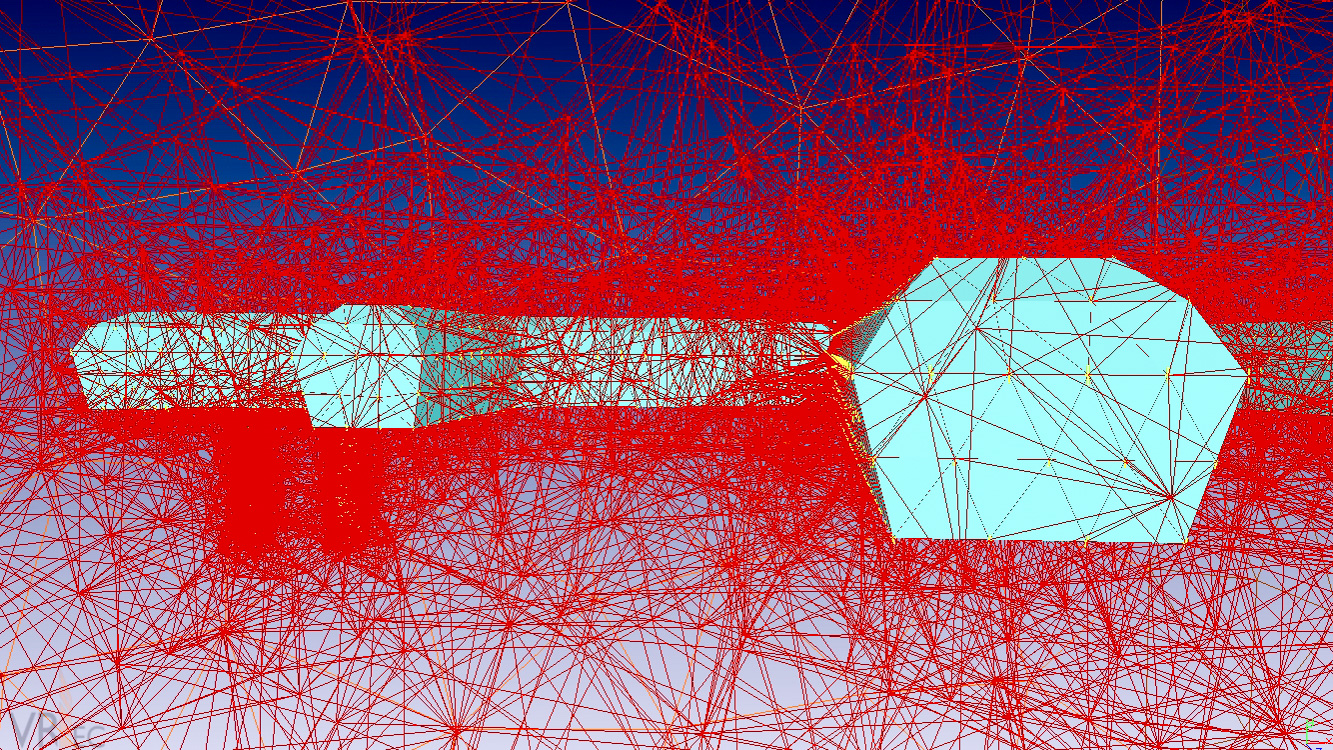
\includegraphics[width=\linewidth]{images/mont-terri.jpg}
\caption{Finite element discretization in the Mont Terri geotechnical laboratory are shown as red lines overlaid on the tunnel system.}
\label{fig:mont-terri}
\end{figure}

\subsection{Gro{\ss}-Sch\"onebeck -- Deep geothermal energy}
\label{grouss-schoenebeck---geothermal-energy}

The Gro{\ss}-Sch\"onebeck site (50\,km north of Berlin, Germany) was established as an in situ laboratory for deep sedimentary geothermal systems. The project aims to develop drilling and stimulation technologies to access deep aquifers in the North German basin where formation temperatures are up to 150\,\celsius. Two wells have been drilled to more than 4\,km depth to form a borehole doublet in permeable porous sandstones and fractured volcanic rocks of the Lower Permian~\cite{zimmermann:geothermal}. Series of hydraulic stimulations resulted in four induced hydraulic fractures to increase the reservoir permeability. The reservoir is also surround by natural fault systems and N- to NE-striking natural faults are expected to serve as main flow path in the current stress field~\cite{bloecher:geothermal}.

\begin{figure}[htb]
  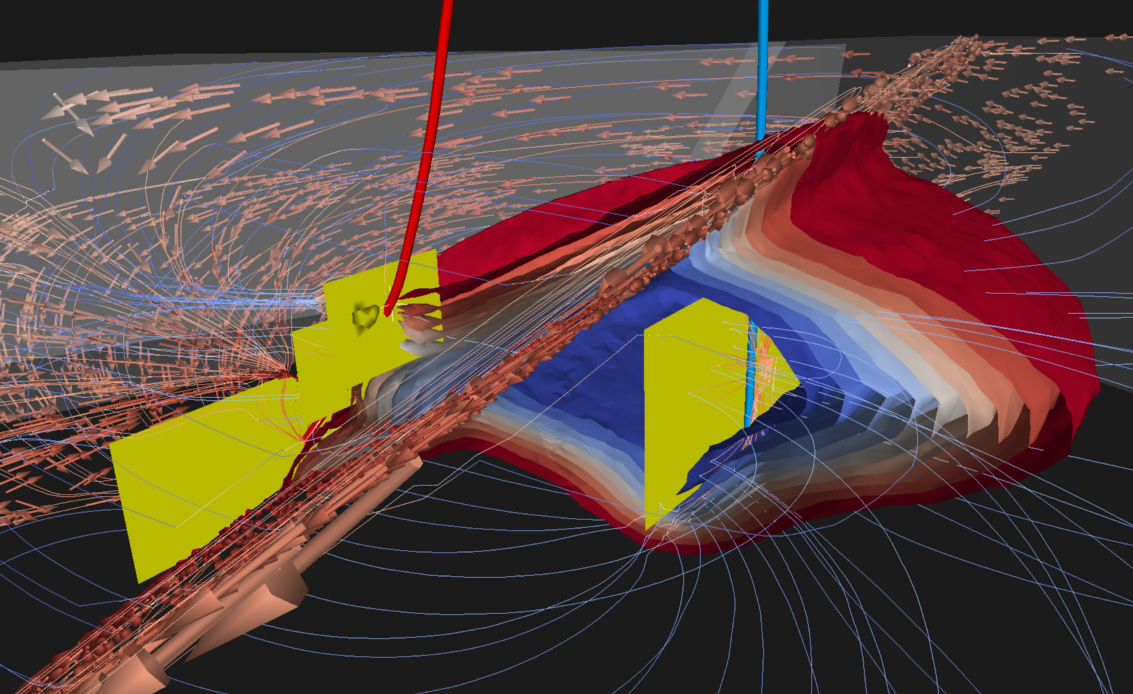
\includegraphics[width=\linewidth]{images/geothermal.jpg}
\caption{Hydraulic behavior visualization with streamlines and arrows representing flow path of injected water and heat transport process represented by iso-surfaces of the cooling front (about 134\,\celsius).}
\label{fig:geothermal}
\end{figure}

One of the ongoing studies in the project is to analyze impacts of the fault zone permeability on reservoir dynamics and overall productivity using a numerical model. The simulated domain includes a horizontal extent of around 5\,km with maximum vertical extension of 594\,m. Based on raster data (for geological layers) and points data (forming faults, induced fractures and well paths), an unstructured grid was generated to represent the complex reservoir structure with more than one million nodes and elements. The simulation takes into account flow and heat transport processes in the reservoir over 100 years assuming injection and production rates of $18\,m^3/h$ and injection temperature of 70\,\celsius. Simulation results in case of highly conductive fault zones were visualized with 3D techniques. The visualization shown in Figure \ref{fig:geothermal} is helpful to understand three dimensional flow path in the complex reservoir structure (mainly along the faults) and subsequent reservoir cooling behavior (convection along the faults with conduction near production). See \cite{zimmermann:geothermal} and \cite{bloecher:geothermal} for more information about the Gro{\ss}-Sch\"onebeck site and the reservoir modeling and~\cite{zehner:uncertainty} for previous work on uncertainty visualization.
%
Numerical modeling with OGS has been used in similar case studies to analyse heat transport and induced phenomena in deep geothermal systems \cite{Kolditz1993467, McDermott2006321, Watanabe2010263}.

%\begin{comment}
\subsection{PROTECT -- Prediction of deformation to ensure carbon traps}
\label{otway-basin---co2-storage}

The \emph{PROTECT} project~\cite{krawczyk:deformation} is a partner project of the Australian \emph{CO2CRC Otway} project~\cite{cook:carbon}. Its aim is to determine the seismic and sub-seismic characteristics of potential fluid migration pathways between reservoir and surface. The goal of this part of the \emph{PROTECT} project that is presented here, was to generate an interactive visualization that combines original geophysical (i.e. seismic data and borehole data) and derived data (i.e.~seismic attributes like coherency), a geological 3D model~\cite{ziesch:geology}, as well as modeling results (from kinematic retro-deformation and geomechanical forward modeling) into an immersive presentation which can be shown on VR display systems.

The first steps were the visualization of our high-resolution, geological 3D model and the 3D seismic data set in ParaView. Conventional 3D P-wave seismic data can image faults with an offset of hundreds of meters down to circa 20 meters. Using seismic attributes (i.e. variance) and visualization of the results within an VR environment, we were able to identify faults with smaller offsets (between 10 and 20 meters). This complements the detailed 3D seismic interpretation and thus helps to identify possible pathways for injected $CO_{2}$.

3D seismics in SEG-Y format cannot be directly imported into \emph{ParaView}, so that a data conversion tool for seismic data was developed~\cite{bilke:simpleseismicreader}. It imports rectilinear-shaped seismic data in a plain text format into \emph{ParaView} using \emph{OpendTect}~\cite{web:opendtect}.

\begin{figure}[htb]
  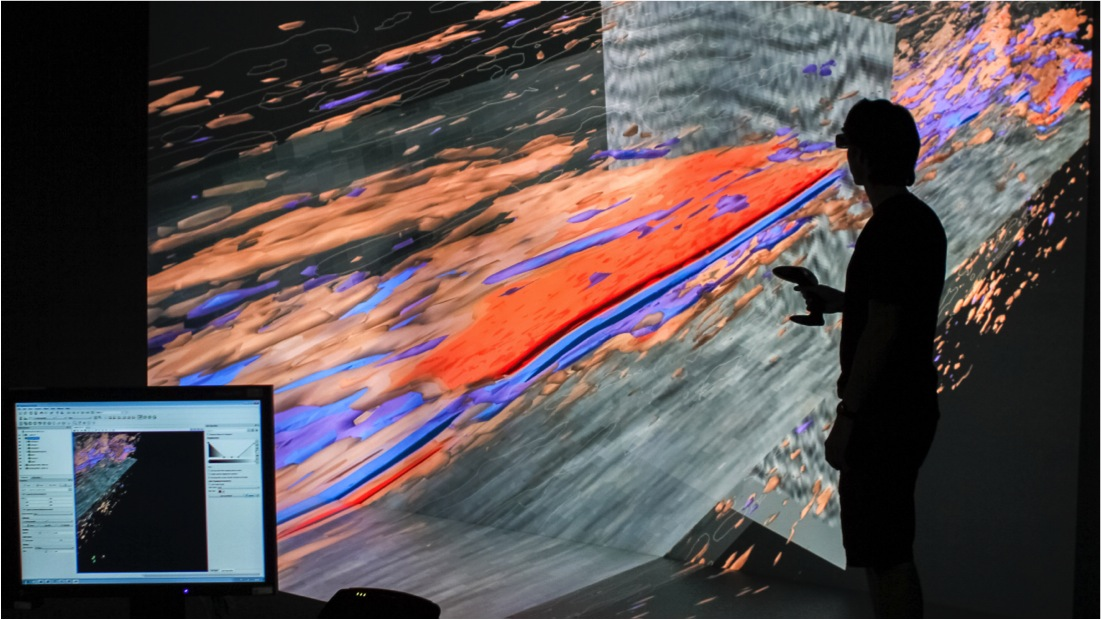
\includegraphics[width=\linewidth]{images/seismic.jpg}
\caption{ParaView running in the VISLab showing a spatial subset and cross-sections of 3D seismic data and isosurfaces of interesting features (modified from \cite{krawczyk:deformation})}
\label{fig:seismic}
\end{figure}
%\end{comment}


\subsection{Thuringian Syncline -- Faults modeling}
\label{thuringian-syncline---faults}

\begin{figure}[htb]
  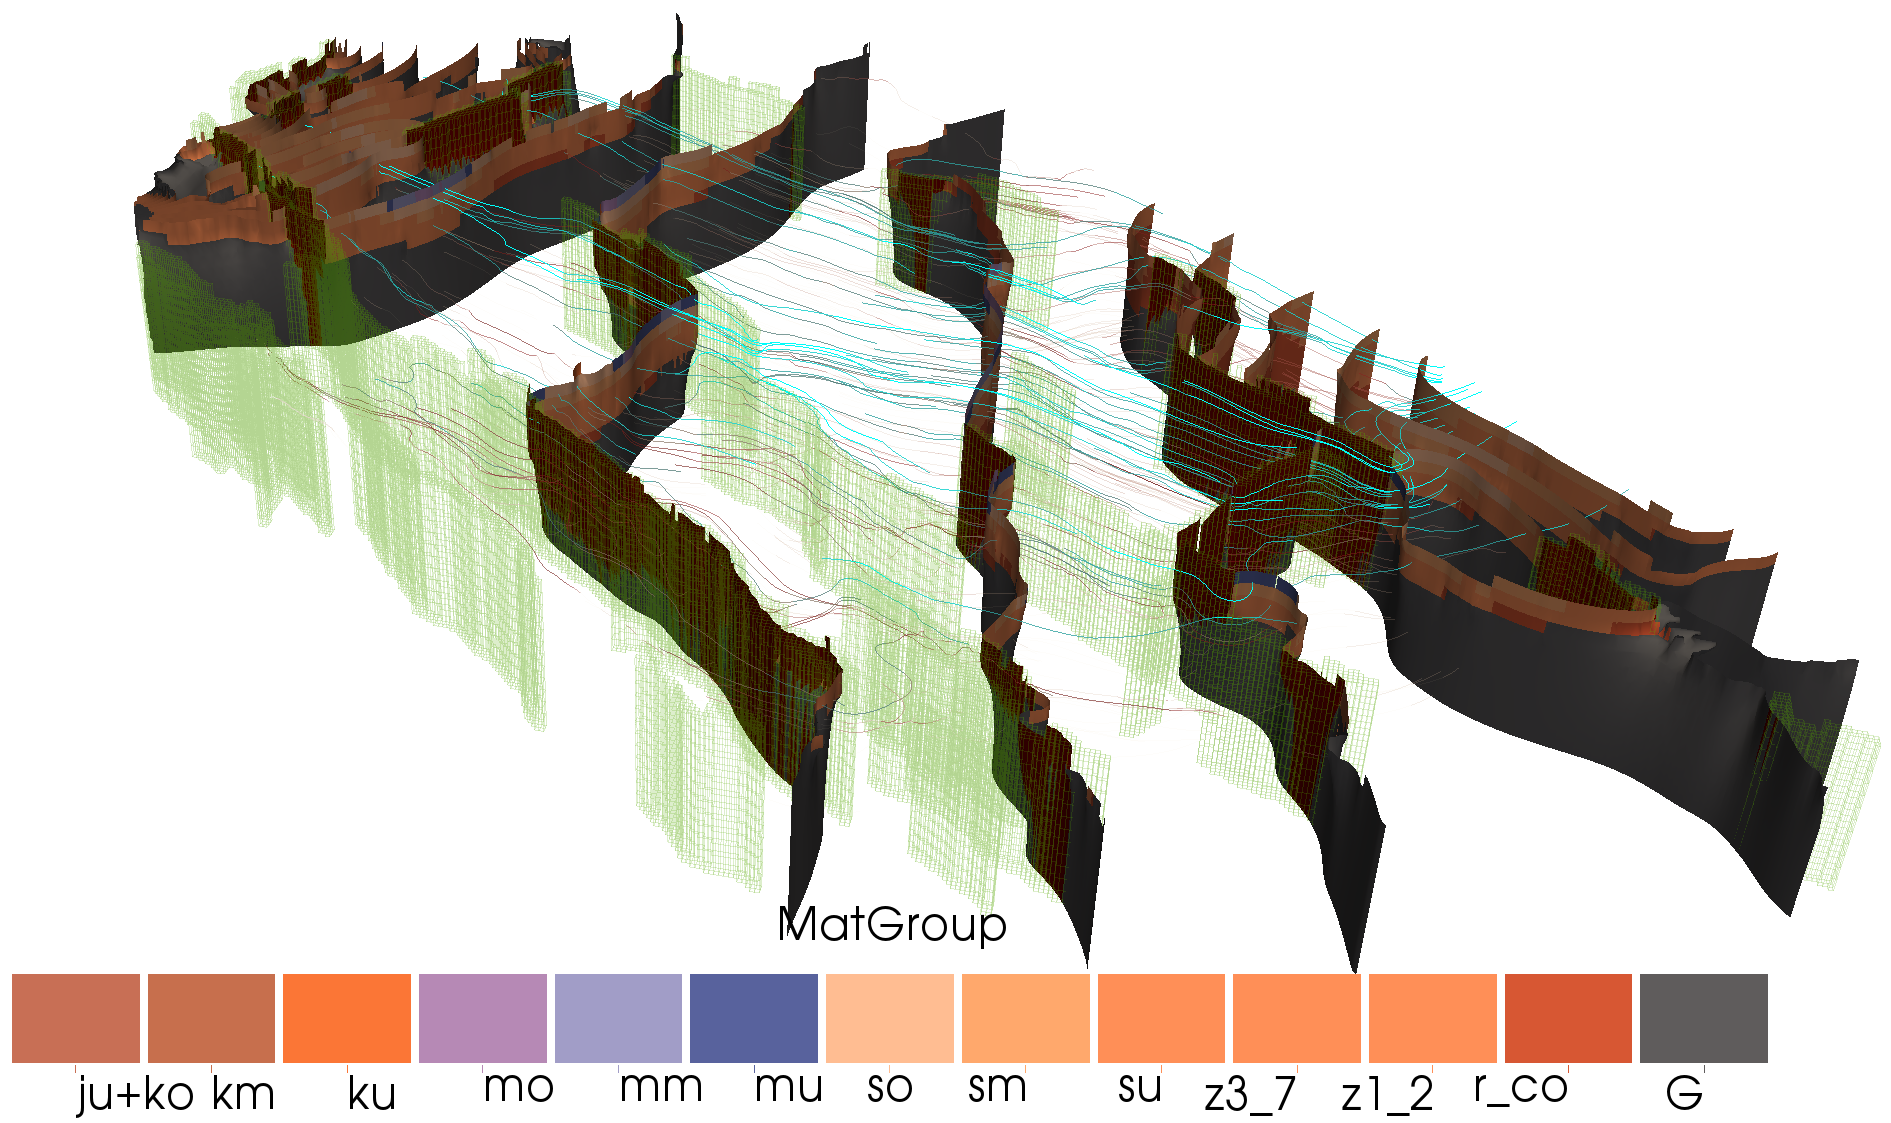
\includegraphics[width=\linewidth]{images/ThuringianSyncline.png}
\caption{Results of prototyp simulation model: Fluid paths (streamlines),
Isosurfaces of hydraulic head colored by stratigraphic layer. The fault zones
are depicted as green colored, wired volumes.}
\label{fig:ThuringianSyncline}
\end{figure}

The \emph{INFLUINS} project investigates the movement of fluids in the
subsurface in the Thuringian Syncline which covers most of the federal state
Thuringia in Germany. Due to the formation history, the syncline contains many
fault zones. The focus of the project is on the flow from the region of the
uppermost soil layer down to the basement at depths in several kilometers
including the effects of fault zones. The geological model is based on a \emph{
GoCad}~\cite{web:gocad} stratigraphic grid.

It covers an area of $11\,800\,\textnormal{km}^2$. The west-north-west to
east-south-east extent is circa $150\,\textnormal{km}^2$, the north-north-east to
south-south-west is circa $80\,\textnormal{km}^2$. The geological model contains 12
stratigraphic layers and 54 fault zones. The visualization is used to get a
better understanding of the course of the stratigraphic layers and faults zones
in the subsurface model. For simulation purposes the challenge is to incorporate the geological model into a finite element mesh~\cite{zehner:gocad}. Also, the elements of the mesh have to meet certain quality criteria such as edge-length-ratio. Visualizations of the mesh and its quality help to identify improvable mesh areas and compare alignment to the original geological model.
Therefore visualization was of great importance to verify particular
steps of the simulation model setup and to
check if boundary conditions were correctly incorporated into the simulation
model. Furthermore the visualization is a valuable tool to interpret the
simulation results of the prototype simulation model as seen in
figure~\ref{fig:ThuringianSyncline}.

%\end{comment}


\subsection{Exploration and management strategies for shallow geothermal energy in residential sites}
\label{shallow-geothermal}

Shallow geothermal energy is a resource-saving alternative to conventional heating and cooling applications in residential buildings~\cite{haehnlein:2013}. Hence, there is a strong increase in large scale geothermal projects, e.g. providing heat for entire residential neighbourhoods~\cite{alkan:2013}. Therefore, novel strategies for shallow geothermal site exploration and management are being developed to promote the sustainable thermal uses of the subsurface. These strategies focus on the enhancement of system efficiency by optimizing system design while minimizing environmental impacts. One application example to test the novel exploration strategy is currently being investigated in an urban neighbourhood in Taucha. For 53 newly developed properties the use of shallow geothermal energy is one option to cover the heating and cooling demand. Different application scenarios are analysed (e.g. open and closed systems, heat storage) to determine induced long-term temperature difference within the soil and groundwater. Heat transport is governed by (hydro-) geological and petrophysical parameters and their variation in space. This makes reliable high resolution model parameterization essential. Three dimensional model simulations and visualizations are a basis for the comprehensive understanding of complex processes within the subsurface. Moreover, this visualization approach is an important tool to identify missing data and to prove consistency of data from different sources~\cite{vienken:2014}. In the case of the Taucha field site, it enhances understanding of temperature anomalies (e.g. heat plume formation) along borehole heat exchanger after different operating times. For instance, temperature changes in 5 to 6 m distance to the borehole heat exchanger can be evaluated, which are officially set distances to neighbouring borehole heat exchangers~\cite{haehnlein:2011}. Furthermore, the visualization is a valuable tool to support scientific outreach and enhance transfer of knowledge~(figure~\ref{fig:geothermal_shallow}). Subsurface characteristics and processes, which are usually inaccessible, are comprehensively presented to stakeholders from public and private sector. Raising awareness of the importance of a sustainable thermal use of the shallow subsurface and showing consequences of its overexploitation will promote the development of novel investigation and management strategies.

\begin{figure}[htb]
  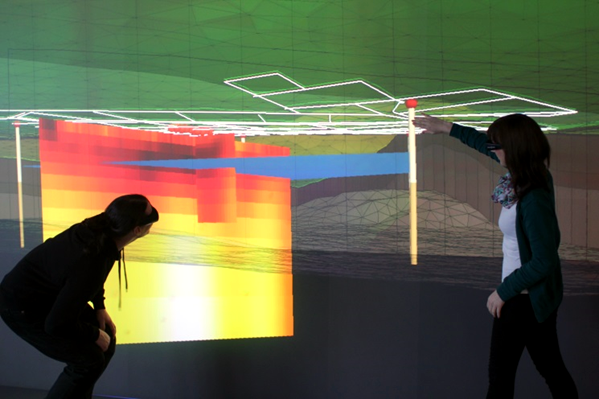
\includegraphics[width=\linewidth]{images/geothermal_shallow.png}
  \caption{Visualization of measured subsurface parameters at a field site in Taucha, Germany (two dimensional geoelectric profiles, horizontal groundwater level, temporary groundwater observation wells, and surface property borders)}
\label{fig:geothermal_shallow}
\end{figure}

\subsection{Climate data -- Visual analysis}
\label{climate-data}

In this case study, simulation data of the \emph{Weather Research and Forecasting} (WRF) model are visualized in combination with observation data from weather stations (i.e.~amount of precipitation at a station) and time independent static data (i.e.~river networks, cities) to analyze it and detect correlations and inconsistencies. The case study area is situated in northern central Europe with an expansion of about 1,300 by 580\,km. It includes various landscapes such as the Alps, lowlands of France, and the English Channel. This area is a common domain for regional weather simulations as it is an area of propagation of frontal systems. The case shows a winter situation on the 28th of January 2012 where the air was moist and cold.

For a detailed analysis of processes such as convection and heat transport, subsets of the area are defined. Figure \ref{fig:wind} shows an example of such a subset, where we concurrently visualized wind fields, mass fraction, humidity and heat fluxes in relation to the digital elevation model. The visualization is used to provide a detailed look at processes and investigate if they have been captured correctly by the model. Different time steps are displayed in an animated manner and the user can i.e.~analyze the development of convection, observe heat transports or study wind fields. The challenge in analyzing these data sets is their highly multivariate character that requires stereoscopic 3D visualization for analysis. The visual combination of simulation, observation, and statical data, which differ in their spatial and temporal resolution, supports the scientists to verify, falsify and generate their hypothesis~\cite{helbig:eesenvirvis}.

\begin{figure}[htb]
  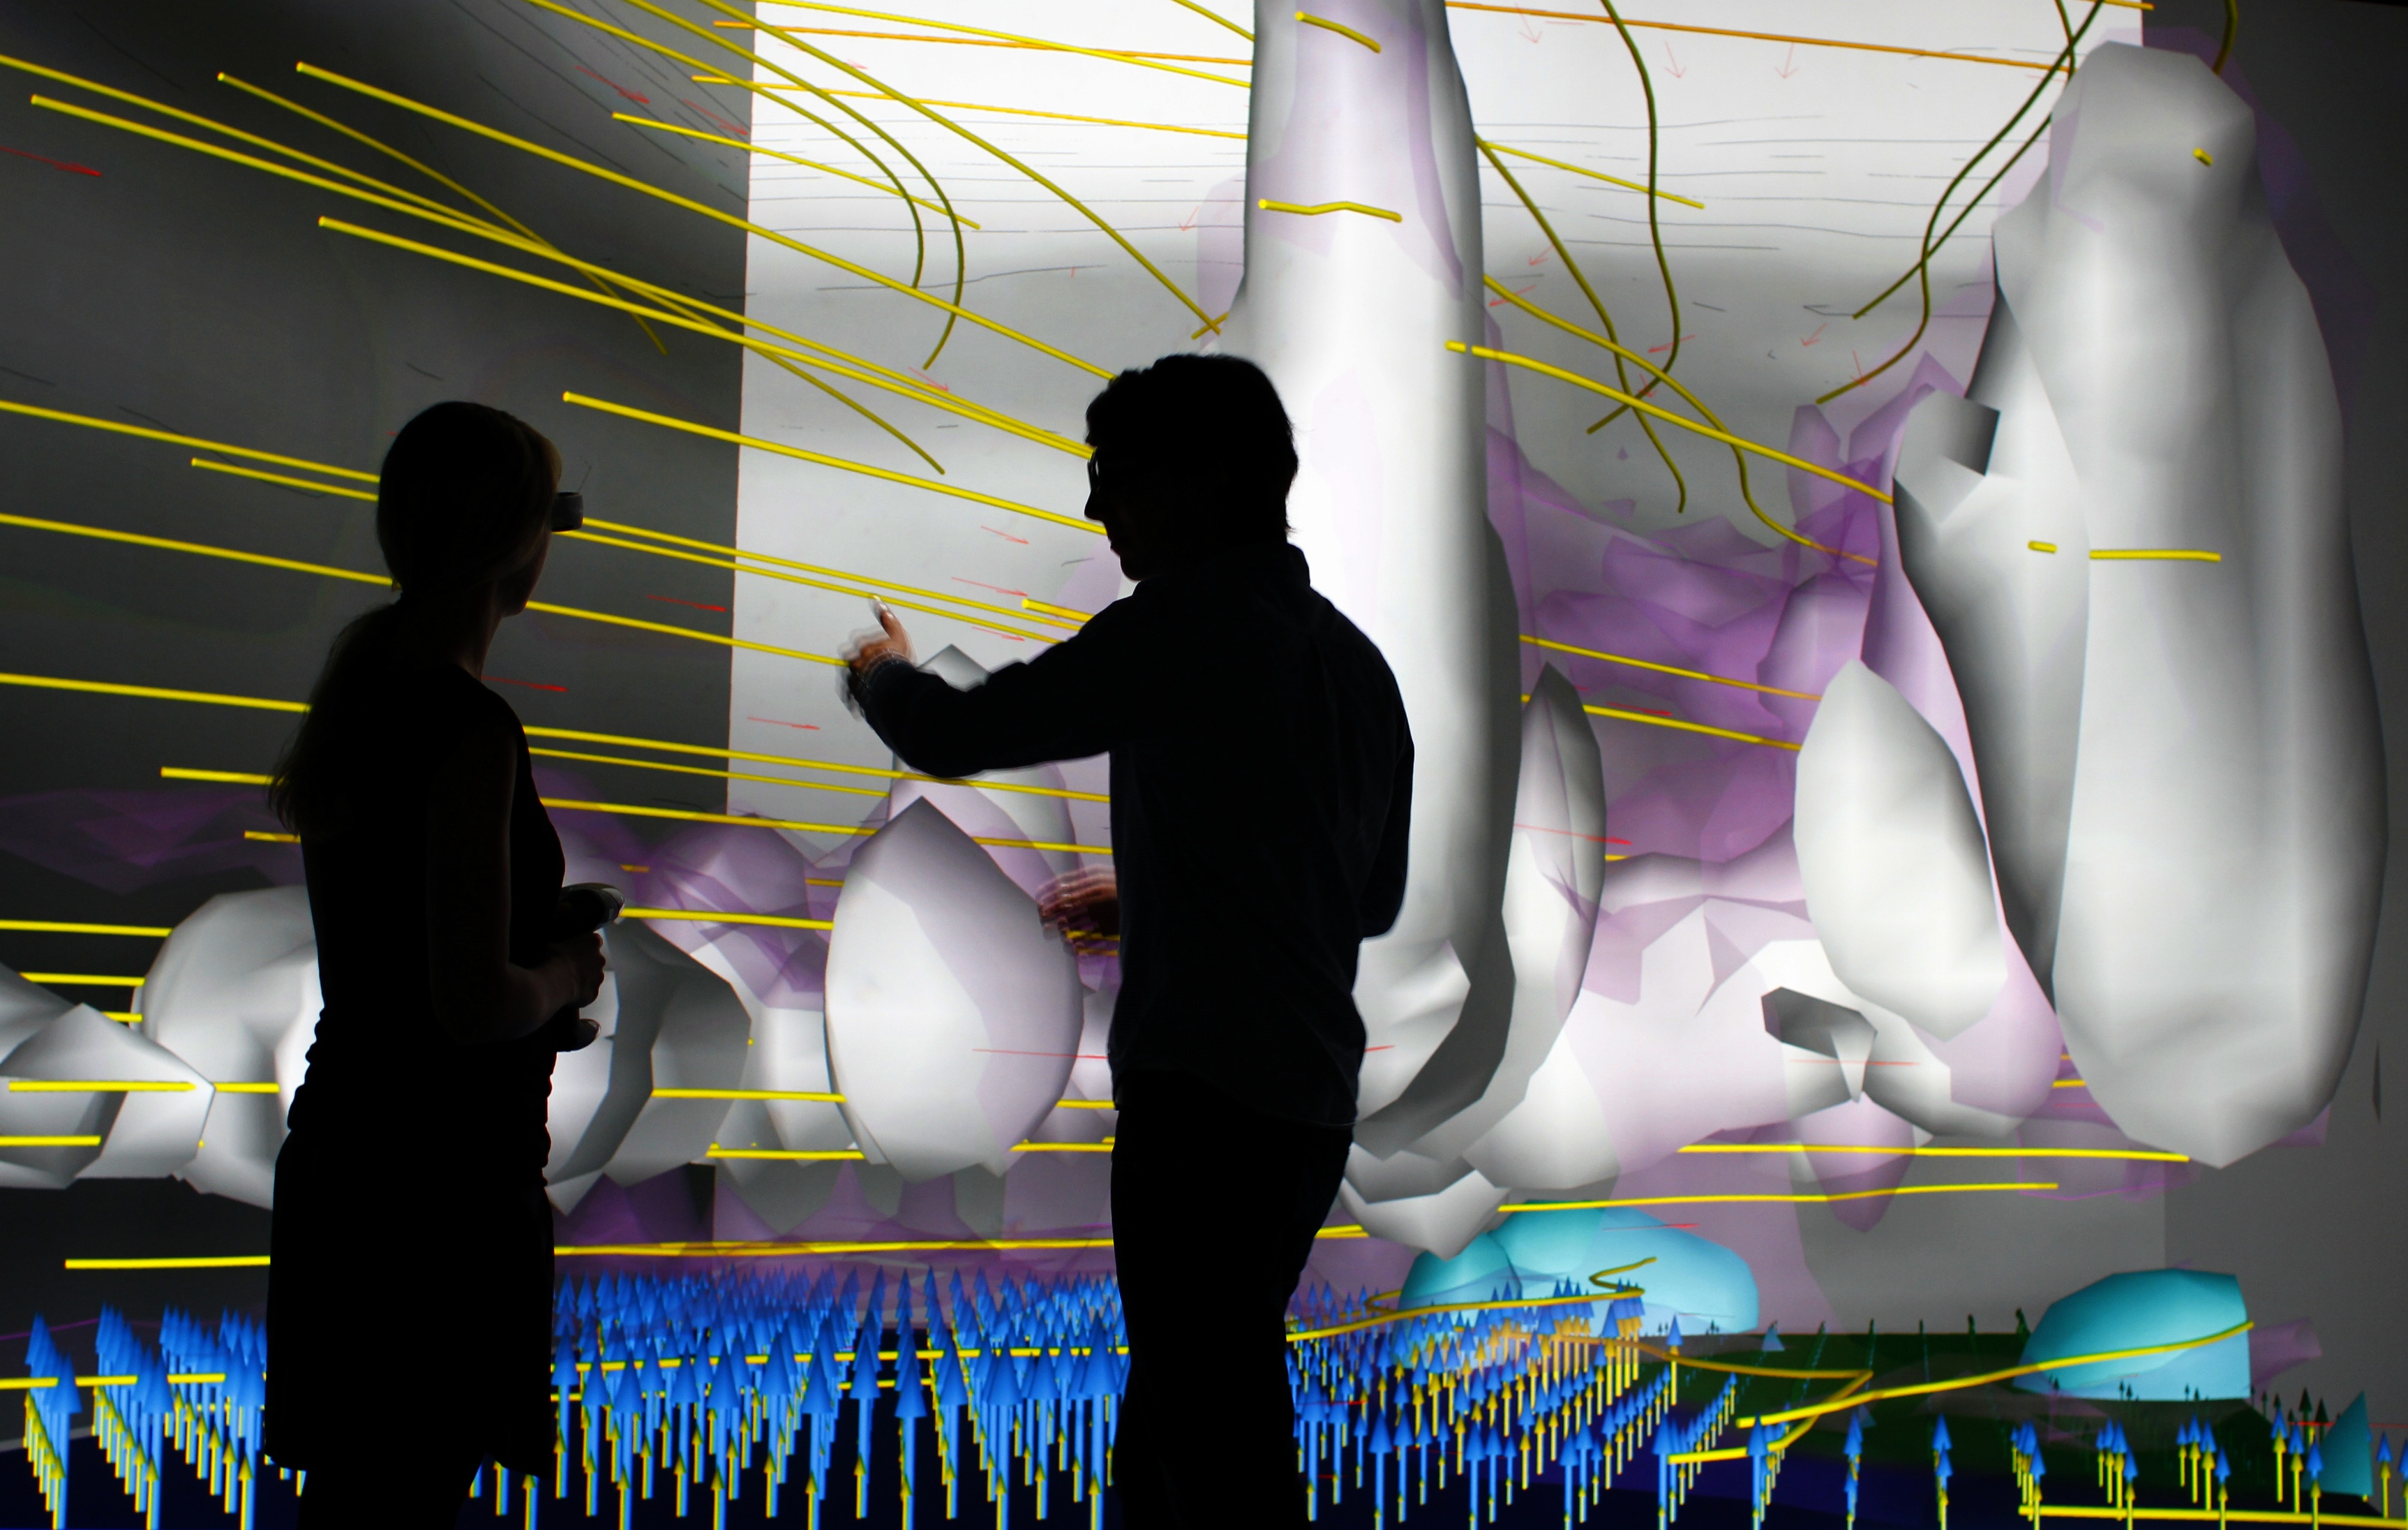
\includegraphics[width=\linewidth]{images/wind.jpg}
  \caption{Climate simulation data visualization showing wind fields (streamlines), mass fraction (white and blue isosurfaces), humidity (slices in the back) and heat fluxes (arrow glyphs on the surface) above the digital elevation model.}
\label{fig:wind}
\end{figure}


\subsection{Pore scale modeling and visualization}
\label{pore-scale}

For a detailed understanding of fluid flow behavior on the pore-scale in unconsolidated sediments simulations of the incompressible Navier-Stokes Equations were performed. The unconsolidated artificial (\emph{in-silico}) sediments were generated with the \emph{SettleDyn} software~\cite{web:SettleDyn} and prepared as input meshes for a finite volume method. The OpenFOAM simulation software~\cite{web:OpenFOAM} was used to obtain a solution of the incompressible Navier-Stokes Equations in the pore network geometry. Additionally, a particle tracking method was applied to simulate particle deposition on the grains' surfaces.

For the particular realization of the randomly generated porous medium we studied the fluid flow patterns in the~pores and distribution of the sticking particles on the surfaces of the grains. Especially the local fluid-flow structures were of interest.

For the visualization of multiple domain boundaries we used a two-sided material rendering technique (described in detail in~\cite{naumov:ees}) obtaining an unobscured view on the~local fluid flow visualization simultaneously keeping the reference to the geometry. Figure~\ref{fig:porescale} depicts the particle visualization with
two-sided materials rendering.

\begin{figure}[htb]
  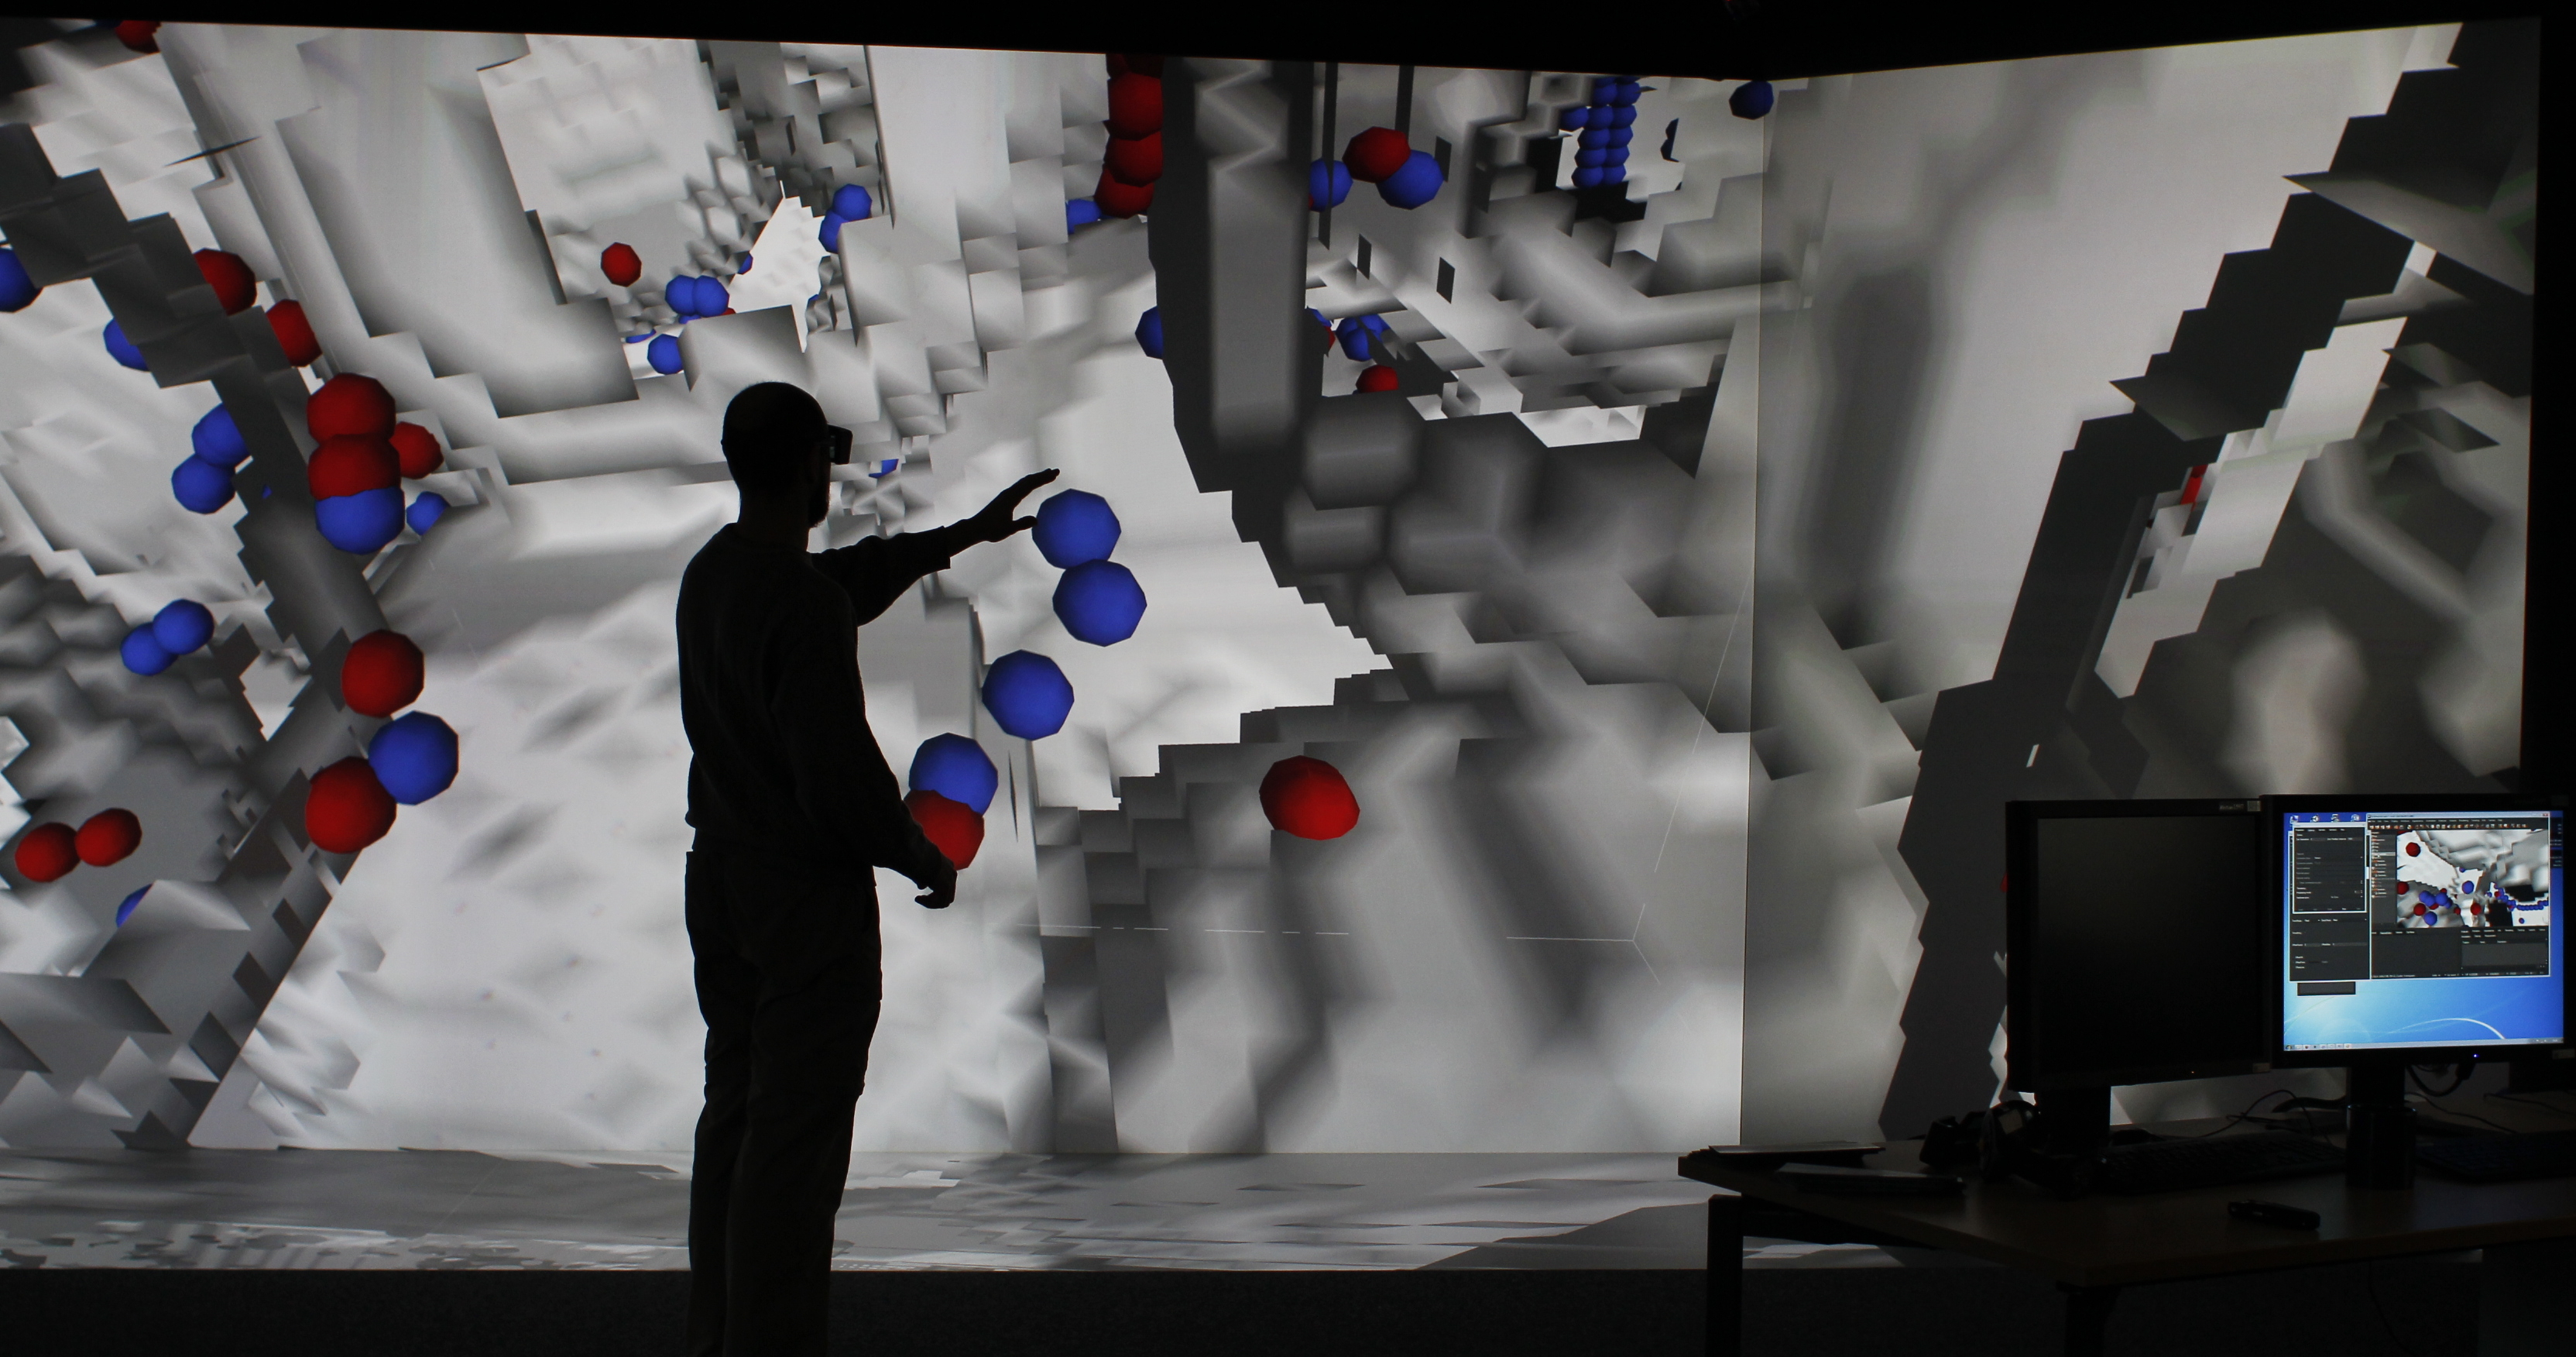
\includegraphics[width=\linewidth]{images/porescale_vislab.jpg}
  \caption{Pore-scale visualization of sticky particles on grains' surfaces.
  The~actor is looking from inside of a~grain looking through it; The~others
  grain's surfaces shown from outside are rendered opaque.}
\label{fig:porescale}
\end{figure}


\begin{comment}
\begin{figure*}
  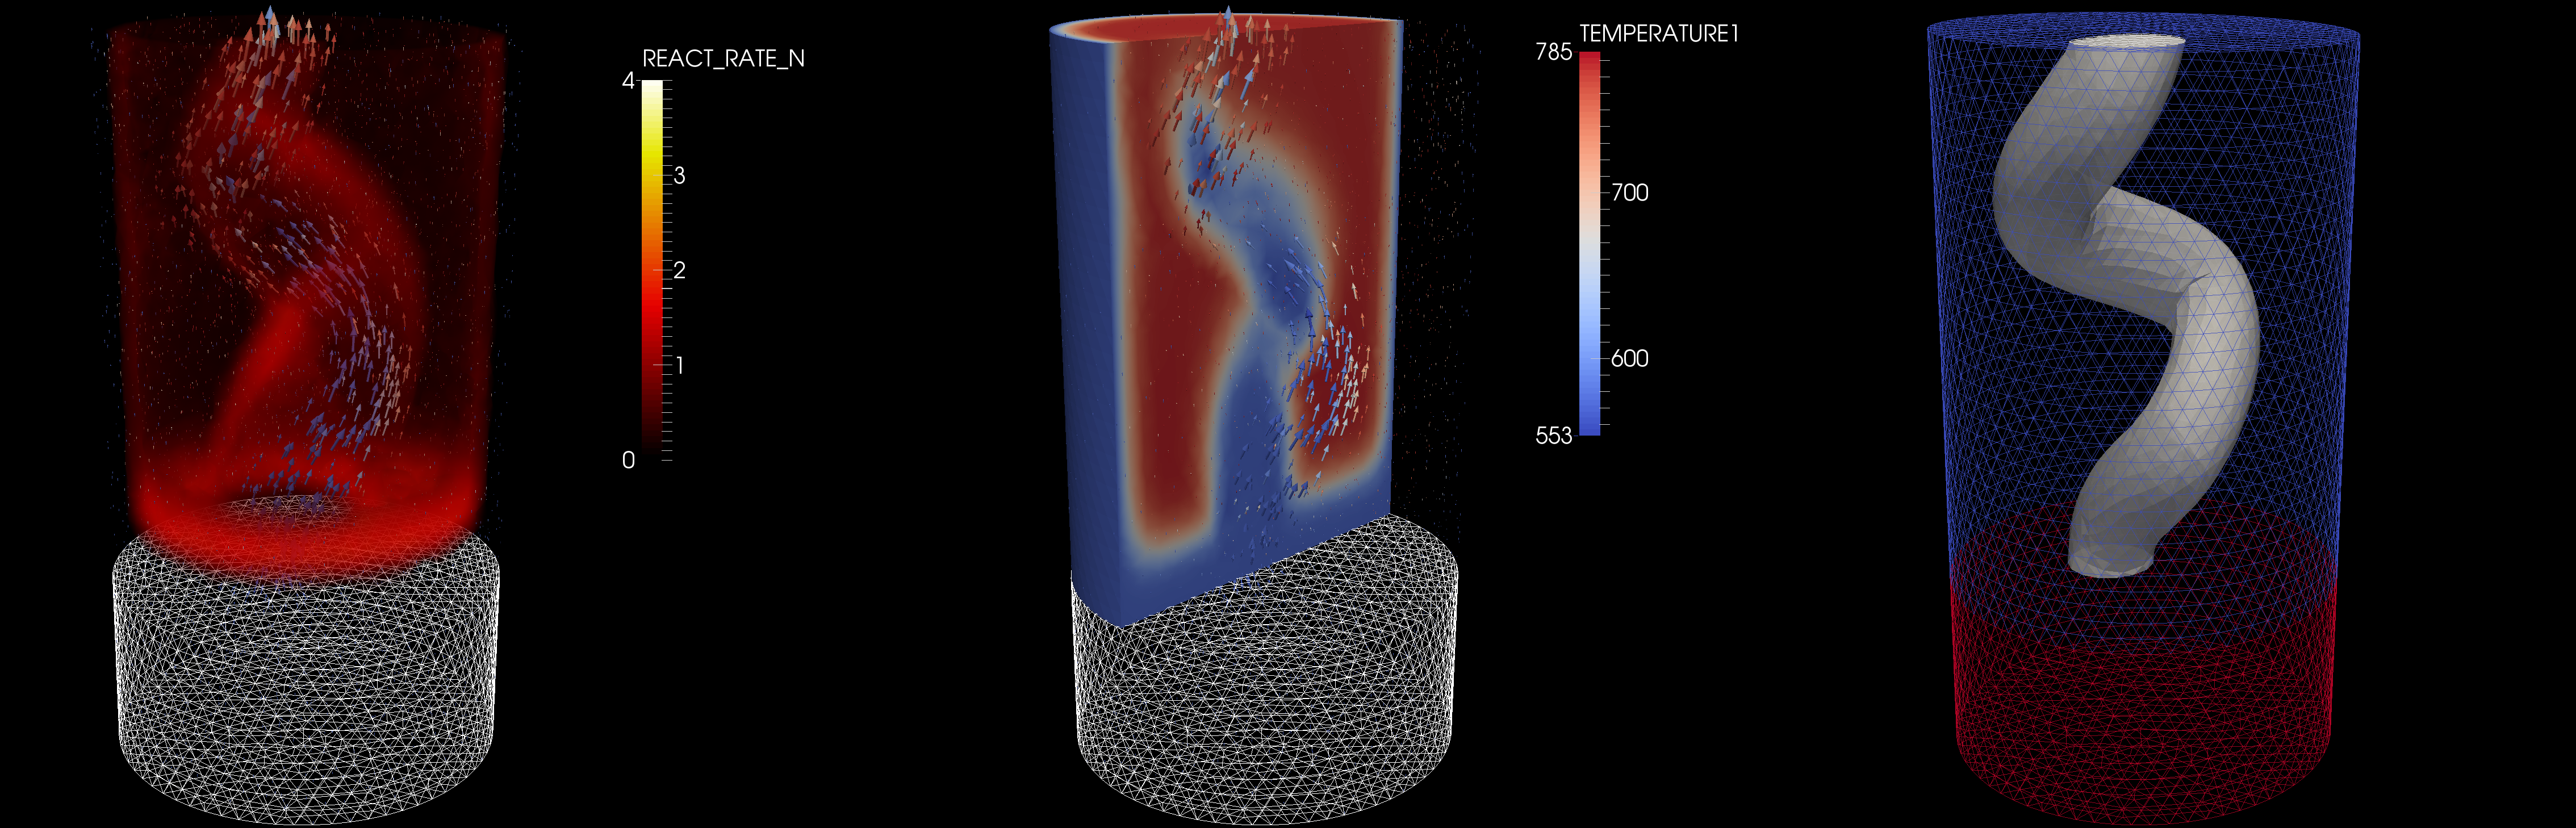
\includegraphics[width=1.0\textwidth]{images/energy_storage.png}
\caption{Paraview visualization of a calcium oxide heat store with an internal heterogeneity (displayed geometrically on the right) during discharge. The volumetric plot on the left displays the reaction rate (kilogram per second) with which the calcium oxide reacts to calcium hydroxide under consumption of water vapor from the gas phase. Arrows indicate the direction and magnitude of the gas flux. The middle plot finally represents a section through the mid-plane of the device and shows the internal temperature distribution in Kelvin. The grid at the bottom represents a porous filter.}
\label{fig:energy_storage}
\end{figure*}
\end{comment}


\subsection{Energy storage}
\label{energy-storage}

A strong coupling between non-equilibrium heat transport at high temperatures, multicomponent mass transport and thermochemical reactions as well as high gradients and nonlinearities are characteristic challenges for numerical models of thermochemical heat storage devices. Such models have been developed for OpenGeoSys in the EWI2 and NUMTHECHSTORE projects and are applied to systems based on metal hydroxides, metal oxides and microporous adsorbents \cite{Nagel2013, Shao2013}. Typically, these devices contain the material in a granular form, which is then permeated by a gas mixture with which the solid reacts under consumption or release of heat depending on the prevailing physicochemical conditions. Simulations are performed with several objectives in mind, e.g. to gain process understanding; to support material development, selection and characterization; to find optimal operation conditions; to estimate device efficiencies and identify efficiency losses.

In some of the considered systems internal heterogeneities can develop. Visualization methods are a useful tool to investigate the complex flow patterns, heat transfer characteristics and chemical reaction profiles that arise as a consequence of these heterogeneities (figure \ref{fig:energy_storage}). This affords the user with an impression of limitations in mass and heat transport and can help to identify locations of, e.g., thermal losses. During cyclic operation (e.g. thermal load buffering) spatially distributed areas of increased or decreased material usage can be identified and linked to thermophysical fatigue mechanisms.

\begin{figure}[htb]
  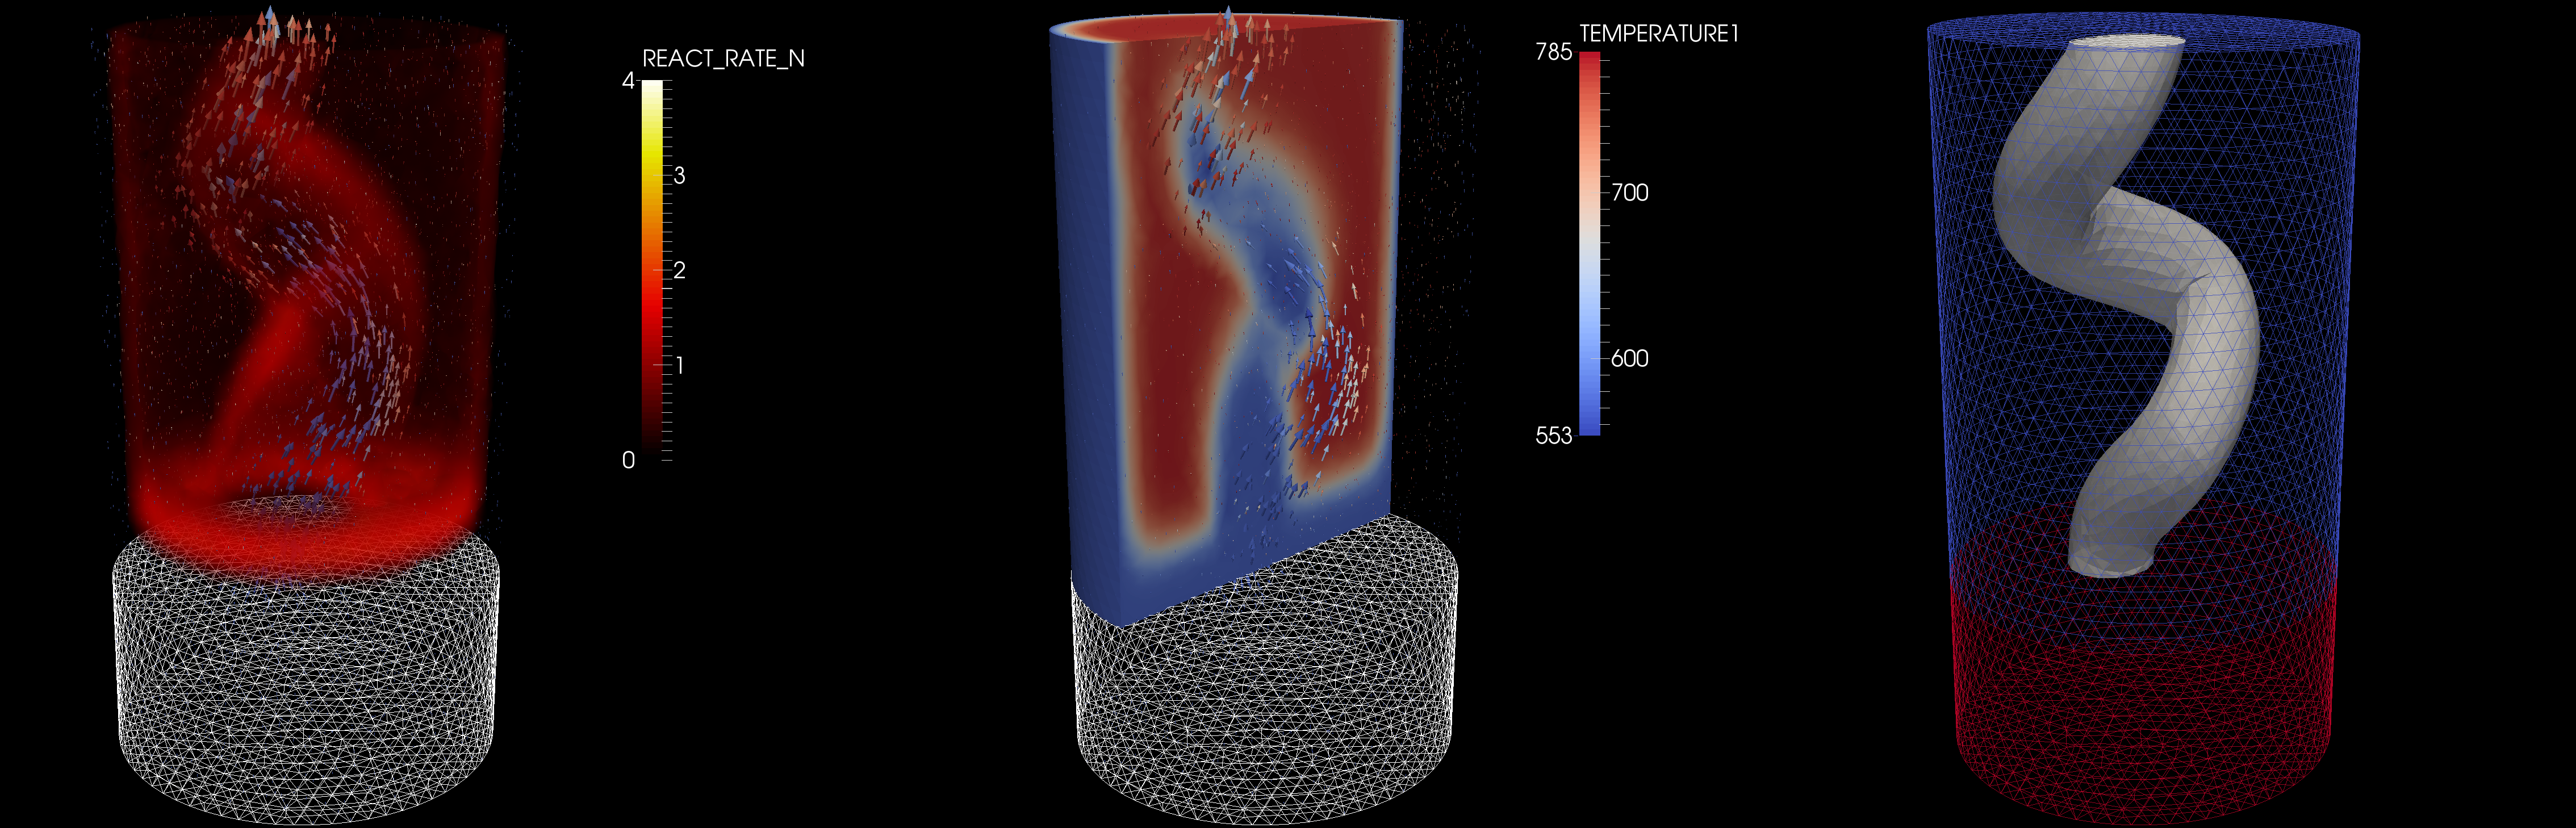
\includegraphics[width=\linewidth]{images/energy_storage.png}
  \caption{Paraview visualization of a calcium oxide heat store with an internal heterogeneity (displayed geometrically on the right) during discharge. The volumetric plot on the left displays the reaction rate (kilogram per second) with which the calcium oxide reacts to calcium hydroxide under consumption of water vapor from the gas phase. Arrows indicate the direction and magnitude of the gas flux. The middle plot finally represents a section through the mid-plane of the device and shows the internal temperature distribution in Kelvin. The grid at the bottom represents a porous filter.}
\label{fig:energy_storage}
\end{figure}


\subsection{Biodiversity in rain forests}
\label{biodiversity-in-rain-forests}

The forests of the earth play an important role in the global carbon cycle. More than 50\,\% of the carbon stored in aboveground vegetation is assumed to be in the tropics~\cite{pan:carbon-sinks}. The dynamics and processes that drive these forest ecosystems are only partly understood. Knowledge about the dynamics of these ecosystems is crucial for ensuring protection and sustainable management of timber, water and other ecological services of these forests. In the working group of Andreas Huth at the Helmholtz Centre for Environmental Research (Department of Ecologial Modelling) the process-based forest growth model \emph{FORMIND}~\cite{huth:1,huth:2} is used to analyze the spatial and temporal forest dynamics by simulating recruitment, mortality and tree growth. With the help of the \emph{VISLab} we are able to visualize the forest growth from a local scale of several square meters up to several hectares. By this, we gain insights into visible and non-visible processes of the forest ecosystem as shown in figure \ref{fig:biodiversity}. Observable processes comprise landslides, fire events and tree falling, whereby invisible processes are included, for example local carbon fluxes. Besides the scientific approach of visualization, it also gives us the opportunity to easily transfer the concept of forest modeling to a broader, mostly non-scientific, community.

\begin{figure}[htb]
  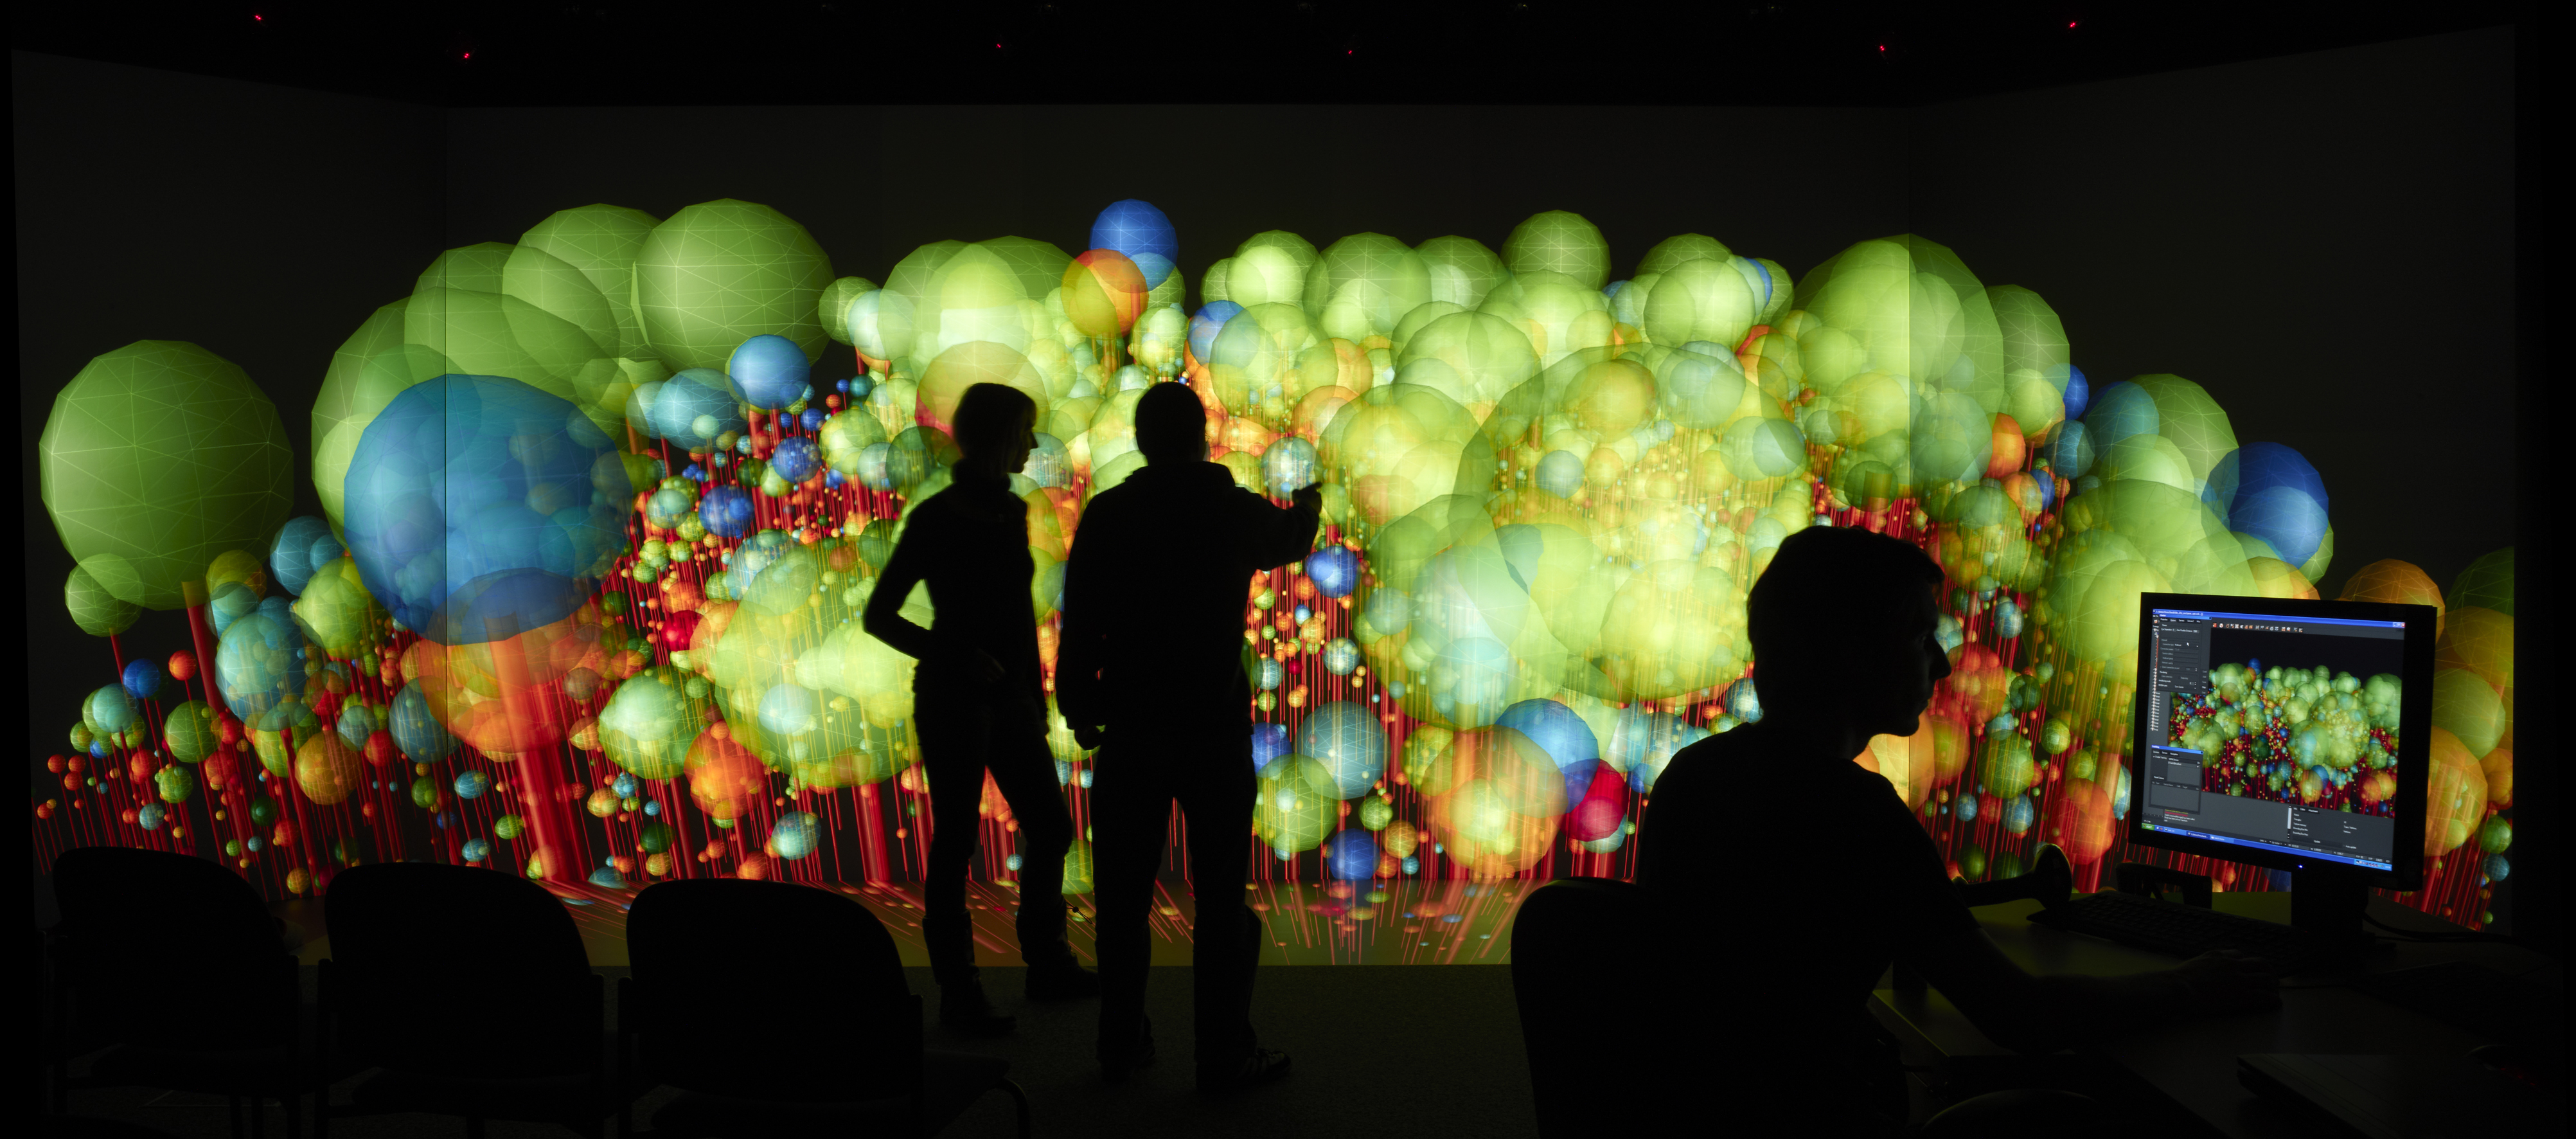
\includegraphics[width=\linewidth]{images/biodiversity.jpg}
\caption{Visualization of a South Ecuadorian montane forest. Different tree crown colors represent the different tree species grouping used in the FORMIND model.}
\label{fig:biodiversity}
\end{figure}


\subsection{Landscape visualization and wind-park planning}
\label{windpark-planning}

We have developed a scenario for applying the \emph{VISLab} to the visualization of landscapes and for interactive tasks, such as interviewing members of the public about their opinions regarding the location and different designs for potential new wind parks. This work has been carried out within the context of a project that aims at finding ways to minimize the conflicts of land use for energy generation using wind-turbines with other uses or with environmental, nature and landscape protection issues.

As a first step a workflow has been developed and a program has been implemented in C++ for the efficient semiautomatic construction of a 3D landscape model from a library of 3D tree models and \emph{GIS} (geographic information systems) data~\cite{zehner:landscape}. The model generated has been constructed using the \emph{OpenSG} scenegraph and could be loaded into \emph{VRED} for displaying it in the \emph{VISLab}. Rendering up to 22\,000 trees, each one consisting of more than 50\,000 polygons at the highest level of detail, required the scene to be highly optimized and to use several rendering tricks, such as the level of detail combined with tree structures, and shading technologies.

\begin{figure}[htb]
  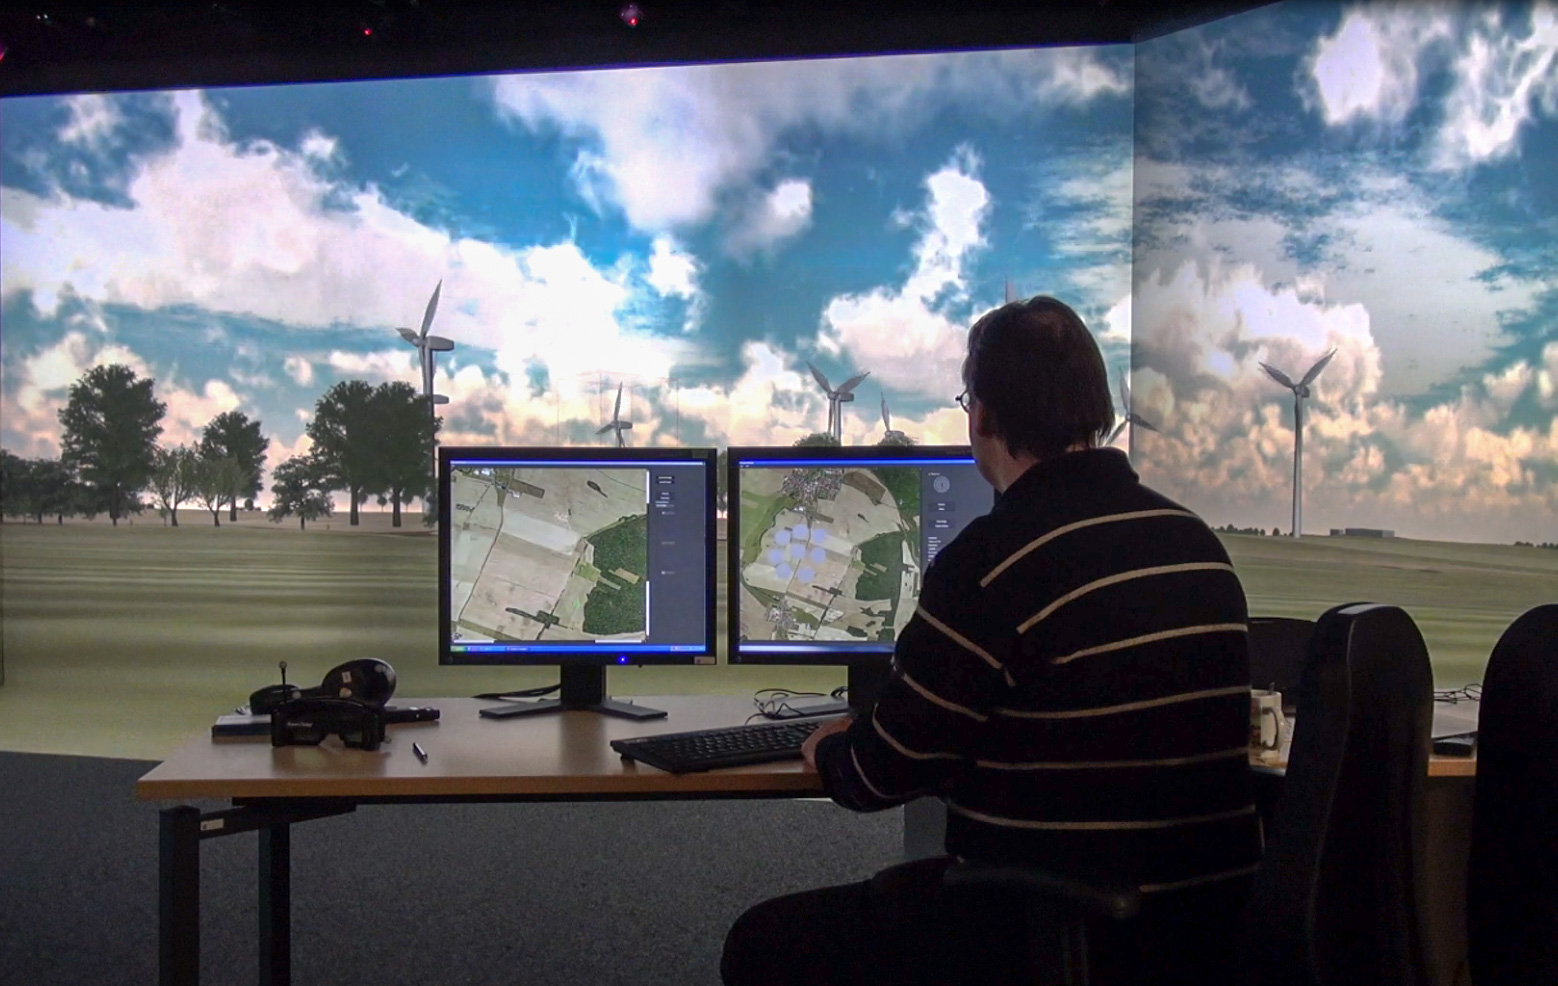
\includegraphics[width=\linewidth]{images/landscape.jpg}
  \caption{Interactive windpark planning in the \emph{VISLab}: The user places wind-turbines and chooses viewing positions on a 2D map on a control pc. The visualization on the large screen is updated in synchronously and can then be further explored using VR interaction techniques.}
\label{fig:landscape}
\end{figure}

As a second step, we developed a scenario for how such a visualization of a landscape could be used to discuss the design of a potential windpark within this landscape~\cite{zehner:windpark}. We extended \emph{VRED}'s user interface, using the \emph{Qt} library~\cite{web:qt}, in order to allow users to navigate through the virtual landscape without getting lost and to enable them to perform simple visually driven planning tasks themselves, such as choosing wind turbines from a set of predefined types and placing it in the field while obeying constraints like the minimum distance of the turbines from each other. As a test of whether novice users could use such a system and in order to get feedback on different setups, we presented it to members of the general public at Leipzig's regional science day, giving the control of the system to the users.

\subsection{Urban environments}
\label{urban-environments}

% TODO put on GitHub and DOI

To help in the creation of urban environment visualizations usable for social sciences and for urban development a procedural\cite{procedural:modelling} building model generator was developed~\cite{bilke:master}. The software called \emph{CityGenerator} allows to procedurally generate building models as well as small city scenes as shown in figure \ref{fig:city} out of simple building blocks such as fa\c{c}ade textures, doors, windows and decoration elements. The user can specify input parameters including the building footprint, building height and designs a template fa\c{c}ade in a graphical user interface. This template fa\c{c}ade is defined by a set of grammatic rules~\cite{procedural:buildings}. The actual model generation is implemented as a \emph{VRED}-plugin allowing for immediate presentation in the \emph{VISLab}. \emph{Level-of-detail} (LOD) techniques ensure a good performance of larger scenes.

\begin{figure}[htb]
  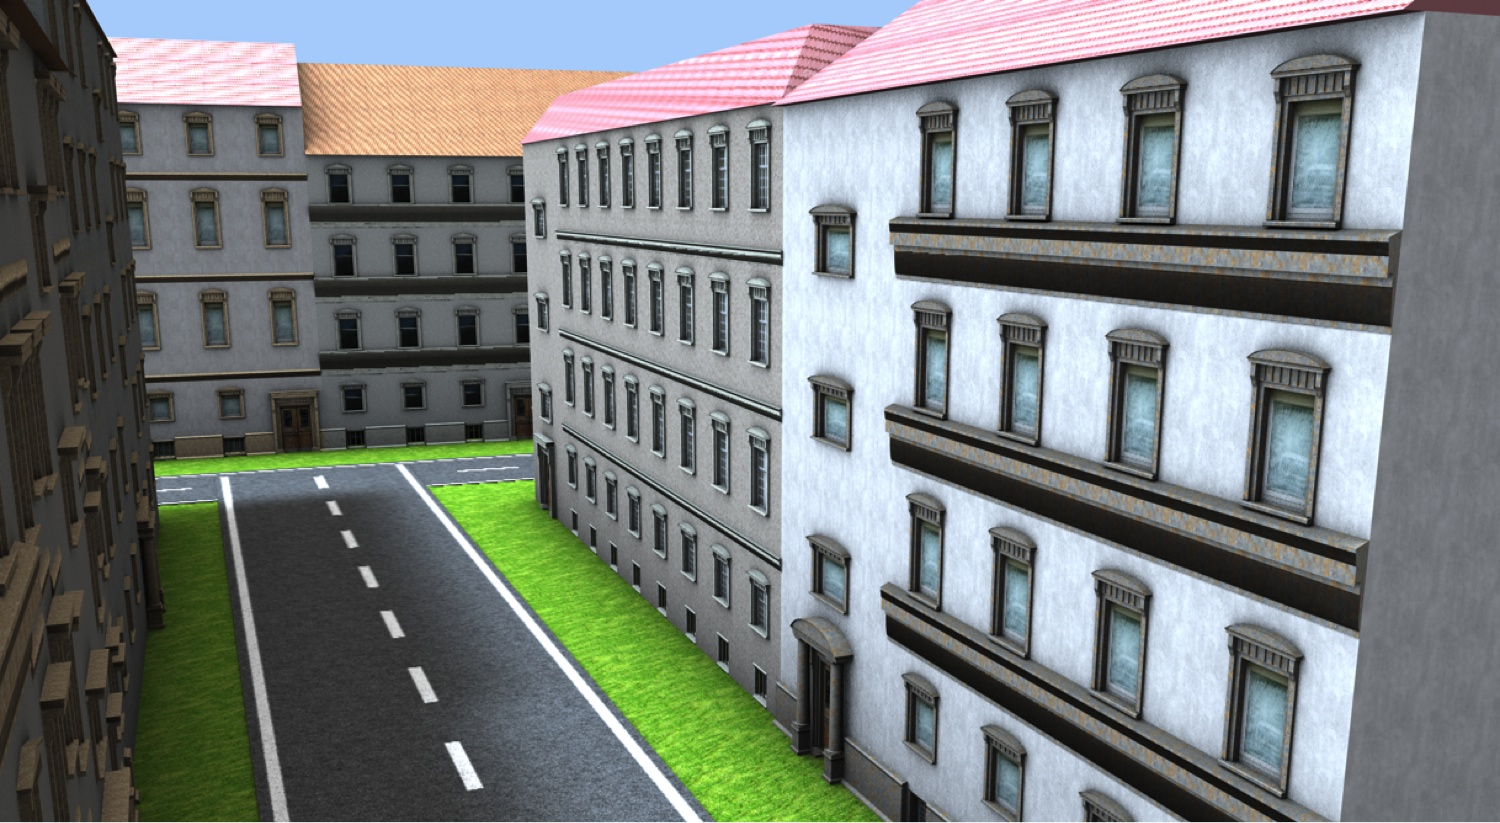
\includegraphics[width=\linewidth]{images/city.jpg}
\caption{Facades and building models in the style of the historic period of promoterism were used as examples to demonstrate the ability of the procedural city generation system.}
\label{fig:city}
\end{figure}

\section{Future work}
\label{future-work}

For the future, we would like to foster the usage of scientific visualization in the daily research work. All software and tools we develop are freely available and open source. Accessibility to these tools is crucial so we are aiming to provide a comprehensive documentation~\cite{web:ogs-docs} which can be enhanced with video tutorials in the future.

For further outreach and education we offer excursions to the \emph{VISLab} for students in environmental sciences, we arrange training courses several times a year and organize workshops at visualization conferences~\cite{web:envirvis}.

To face the challenge to visualize increasingly complex models and simulations, especially in the field of high-performance computing (HPC), we will integrate visualization methods into simulation codes. A simplification of the technical setup of the \emph{TESSIN VISLab} will unlock more fields of applications.

\subsection{In-situ visualization}
\label{in-situ-visualization}

\emph{In-situ}- or \emph{Co}-visualization allows to create result analysis and visualization as a part of the simulation process. By observing the simulation process it is possible to detect errors in the input data early. The user can then cancel the simulation, adapt the input data and restart the simulation. This saves computing time, decreases the workload of scientists and give rise to an effective iterative process of refining and adapting the simulation. Because the \emph{in-situ} visualization can be run without user interaction, it can also be useful for software quality management and benchmarking by automatically comparing visualization output and analyzed data between different program versions.

Normally, the simulation process is divided into four parts: during \emph{preprocessing} the raw input data is transformed and validated. The \emph{model setup} configures the involved model for the given problem appropriately. Typically the \emph{simulation} step produces large amounts of result data, especially in the field of coupled process simulations, which are then processed and analyzed in the \emph{postprocessing} step to reduce data by significance and to identify interesting aspects. Usually the postprocessing takes place on frontend-nodes of the HPC system or on the users machine where storage capacity may be limited. In the latter case all result data have to be transfered over the computer network which can be the limiting factor in various applications. The analyzed data as the outcome of the postprocessing step can be much smaller than the simulation result data.

Therefore, the postprocessing should become integrated into the simulation itself to avoid the communication bottleneck by transferring the analyzed data only and to allow users to monitor their simulated processes to ensure reasonable behavior.

We started using the library \emph{Catalyst}~\cite{web:catalyst} for integration of such an \emph{in-situ} visualization system into \emph{OpenGeoSys}. \emph{Catalyst} is an extension of \emph{VTK} / \emph{ParaView}. On the basis of a representative example data set the user defines a visualization pipeline (either by a script or interactively in \emph{ParaView}) which is then executed after defined time step intervals of the simulation. During simulation time the user gets processed data as a result of the visualization pipeline, images of the visualization and an interactive remote visualization in \emph{ParaView}.

Furthermore, it should be possible to view the remote visualization in the VR environment of the \emph{VISLab}, which is also connected to the HPC system of the UFZ via a fast computer network (\emph{Infiniband}).

\subsection{Simplified hardware setup}
\label{simplified-hardware-setup}

Our current hardware setup limits the usable 3D applications to software which can be run in parallel and synchronized on a computer cluster. This rules out the usage of commonly used software in environmental sciences such as geographic information systems. Novel high resolution projectors can help us to reduce the number of projectors for our display from 13 to 8 in which the main screen is driven by one 4K (Ultra HD resolution) projector instead of six SXGA projectors while also increasing the pixel count by approximately 30\,\%. This allows the usage of every 3D enabled application when disclaiming the projection on the floor and side screens. Also startup times of the display will be much faster and overall system reliability is improved. The technical implementation of such a setup in combination with the remaining projectors on the floor and side screens is currently under review. An additional wireless presentation system~\cite{web:clickshare} entitles even people not familiar with the display system a straightforward usage of it.

%%%%%%%%%%%%%
%% ENDCONTENT
%%%%%%%%%%%%%


\begin{acknowledgements}
The intention of this work is a compilation of case studies which have been carried out in the visualization laboratory \emph{TESSIN VISLAB} over the last years comprising different disciplines in environmental sciences (without claiming completeness). The authors would like to thank Thomas Kalbacher, Karsten Rinke, Benny Selle, Feng Sun and Nico Trauth for providing some of the data sets presented in the case studies. We thank Leslie Jakobs for the improvement of the manuscript concerning clarity and language.

We acknowledge the participation of Departments of the Helmholtz Centre for Environmental Research UFZ in supporting several interdisciplinary case study visualizations, Catchment Hydrology (CATHYD), Computational Hydrosystems (CHS), Hydrogeology (HDG), Groundwater Remediation (GWS), Monitoring and Exploration Technologies (MET), Ecosystem Analysis (OESA), Lake Research (SEEFO).

We are very grateful to our external cooperation partners for data provision and fruitful discussion to improve visualization as a practical and useful tool for applied research, Federal Institute for Geosciences and Natural Resources (BGR), German Research Centre for Geosciences (GFZ), Leipzig University of Applied Sciences (HTWK), Leibniz Institute for Applied Geosciences (LIAG), University of Leipzig, Technische Universit\"at Dresden, Technische Universit\"at Freiberg.
This work was sponsored in part by the Australian Commonwealth Government through the Cooperative Research Centre for Greenhouse Gas Technologies (CO2CRC). PROTECT is funded through the ''Geotechnologien'' Programme (grant 03G0797). We acknowledge the support by the NUMTHECHSTORE project in cooperation with the Institute of Chemical Technology, University Leipzig, and the EWI2 project in cooperation with the Institute of Technical Thermodynamics, German Aerospace Center (DLR).


Further acknowledgements to particular project funding are referred to in the individual papers cited for the case studies presented in this article.
\end{acknowledgements}

% BibTeX users please use one of
%\bibliographystyle{spbasic}      % basic style, author-year citations
\bibliographystyle{spmpsci}       % mathematics and physical sciences
%\bibliographystyle{spphys}       % APS-like style for physics
\bibliography{vislab}   % name your BibTeX data base

\end{document}
% end of file template.tex

